\documentclass[12pt, a4paper]{report}

% --- PACKAGES ---
\usepackage[utf8]{inputenc}
\usepackage[T1]{fontenc}
\usepackage{geometry}
\geometry{margin=2.5cm}
\linespread{1.3}

\usepackage{graphicx}
\graphicspath{{../assets/screenshots/}{../assets/demo-screenshots/}}

\usepackage{booktabs}
\usepackage{tabularx}
\usepackage{longtable}
\usepackage{amsmath, amssymb}

\usepackage{listings}
\usepackage{xcolor}

\usepackage{tikz}
\usetikzlibrary{shapes.geometric, arrows.meta, positioning, calc}

\usepackage{hyperref}
\hypersetup{
    colorlinks=true,
    linkcolor=blue,
    citecolor=blue,
    urlcolor=blue,
    pdftitle={FPLIP Academic Report},
    pdfauthor={FPLIP Project Team}
}

\usepackage[backend=biber, style=ieee]{biblatex}
\addbibresource{references.bib}

\usepackage{fancyhdr}
\pagestyle{fancy}
\setlength{\headheight}{15pt}
\fancyhf{}
\rhead{\leftmark}
\lhead{FPLIP Academic Report}
\cfoot{\thepage}

% --- LISTINGS CONFIGURATION ---
\definecolor{codegreen}{rgb}{0,0.6,0}
\definecolor{codegray}{rgb}{0.5,0.5,0.5}
\definecolor{codepurple}{rgb}{0.58,0,0.82}
\definecolor{backcolour}{rgb}{0.96,0.96,0.96}

\lstdefinestyle{sqlstyle}{
    language=SQL,
    backgroundcolor=\color{backcolour},
    commentstyle=\color{codegreen}\itshape,
    keywordstyle=\color{blue}\bfseries,
    numberstyle=\tiny\color{codegray},
    stringstyle=\color{codepurple},
    basicstyle=\ttfamily\footnotesize,
    breakatwhitespace=false,
    breaklines=true,
    captionpos=b,
    keepspaces=true,
    numbers=left,
    numbersep=5pt,
    showspaces=false,
    showstringspaces=false,
    showtabs=false,
    tabsize=2,
    frame=single
}

\lstdefinestyle{pythonstyle}{
    language=Python,
    backgroundcolor=\color{backcolour},
    commentstyle=\color{codegreen}\itshape,
    keywordstyle=\color{purple}\bfseries,
    numberstyle=\tiny\color{codegray},
    stringstyle=\color{teal},
    basicstyle=\ttfamily\footnotesize,
    breakatwhitespace=false,
    breaklines=true,
    captionpos=b,
    keepspaces=true,
    numbers=left,
    numbersep=5pt,
    showspaces=false,
    showstringspaces=false,
    showtabs=false,
    tabsize=2,
    frame=single
}

\lstdefinestyle{yamlstyle}{
    backgroundcolor=\color{backcolour},
    commentstyle=\color{codegreen}\itshape,
    keywordstyle=\color{blue}\bfseries,
    numberstyle=\tiny\color{codegray},
    stringstyle=\color{orange},
    basicstyle=\ttfamily\footnotesize,
    breakatwhitespace=false,
    breaklines=true,
    captionpos=b,
    keepspaces=true,
    numbers=left,
    numbersep=5pt,
    showspaces=false,
    showstringspaces=false,
    showtabs=false,
    tabsize=2,
    frame=single,
    morekeywords={version, models, columns, tests, name, description, constraints, type}
}

% --- TITLE PAGE ---
\begin{document}

\begin{titlepage}
    \centering
    \vspace*{1cm}
    
    {\Large \textbf{NATIONAL SCHOOL OF APPLIED SCIENCES (ENSA SAFI)}}\\[0.3cm]
    {\large Department of Computer Science \& Industrial Engineering}\\[0.2cm]
    {\large Master of Engineering in Data Engineering \& Artificial Intelligence (IDIA)}\\[1.5cm]
    
    \rule{\linewidth}{0.5mm}\\[0.4cm]
    {\huge \textbf{Factory Performance \& Loss Intelligence Platform (FPLIP)}}\\[0.3cm]
    {\large \textit{A Contract-Governed, Zero-Cost Data Lakehouse with Operational Workflow, Business Intelligence, and Grounded AI Analytics}}\\[0.4cm]
    \rule{\linewidth}{0.5mm}\\[1.5cm]
    
    \begin{minipage}{0.45\textwidth}
        \begin{flushleft} \large
            \textbf{Author:}\\
            Data Engineering Team\\
            IDIA Master Candidate
        \end{flushleft}
    \end{minipage}
    \begin{minipage}{0.45\textwidth}
        \begin{flushright} \large
            \textbf{Academic Year:}\\
            2025--2026\\[0.1cm]
            \textbf{Deliverable:}\\
            Final Internship Project
        \end{flushright}
    \end{minipage}
    
    \vfill
    {\large August 2026}
\end{titlepage}

% --- ABSTRACT ---
\begin{abstract}
Manufacturing enterprises lose substantial operational efficiency through fragmented logs, unquantified downtime, and unmitigated scrap rates. The Factory Performance \& Loss Intelligence Platform (FPLIP) addresses this challenge by establishing a production-grade, zero-cost data platform that transforms raw factory logs into real-time Overall Equipment Effectiveness (OEE) metrics, scrap root-cause attribution, and automated operational workflows. Built under strict zero-cost cloud constraints using the GCP BigQuery Sandbox, FPLIP implements an end-to-end Medallion Architecture (Bronze, Silver, and Gold) orchestrated by dbt and Apache Airflow via GitHub Actions. Pre-ingestion data contracts enforce schema compliance before ingestion, while idempotent partition-decorator loads guarantee reproducible execution. Hand-rolled DDL pattern for Slowly Changing Dimensions (SCD Type 2) overcomes cloud sandbox DML execution blocks without requiring MERGE operations. 

Downstream, FPLIP exposes a lightweight FastAPI serving tier with 4-hour in-memory TTL caching, feeding an operational Laravel (PHP) application equipped with Role-Based Access Control (RBAC) and an investigation lifecycle (detect $\rightarrow$ investigate $\rightarrow$ assign $\rightarrow$ fix $\rightarrow$ close). Visual analytics are delivered through a 4-row storytelling dashboard on Apache Superset. An interpretability-focused Logistic Regression machine learning model predicts scrap risk per run, while a grounded AI Copilot utilizes a tool-calling architecture restricted to four deterministic functions to eliminate hallucination risks. Validated through cold-restart testing, rigorous dbt test suites, and ephemeral per-PR CI/CD dataset isolation, FPLIP demonstrates a robust template for contract-governed, agent-safe manufacturing lakehouses under real-world infrastructure boundaries.
\end{abstract}

\tableofcontents
\listoffigures
\listoftables

% --- CHAPTER 1: INTRODUCTION ---
\chapter{Introduction}
\label{chap:introduction}

\section{Business Context}
Modern discrete manufacturing facilities operating multi-line production environments---such as concrete block pressing, pavement block molding, and zellige tile fabrication---face intense pressure to optimize operational throughput and minimize scrap. Despite the proliferation of digital sensors and manual data entry terminals, manufacturing data frequently remains trapped in raw CSV export logs and isolated operational tables. Operational leaders are left without continuous visibility into Overall Equipment Effectiveness (OEE), scrap root causes, or loss attribution.

In greenfield industrial deployments, establishing a modern data lakehouse often encounters severe budget constraints and infrastructure access hurdles. Enterprise data projects frequently stall due to high cloud resource costs, complex billing requirements, and lengthy procurement cycles. This project addresses the fundamental challenge of engineering a production-ready, contract-governed, and fully automated manufacturing data platform executed entirely within a zero-cost infrastructure environment (GCP BigQuery Sandbox), serving operational managers and line technicians seamlessly.

\section{Problem Statement}
Before FPLIP, factory managers and quality control technicians lacked an integrated analytical system to answer critical operational questions:
\begin{enumerate}
    \item \textbf{Loss Visibility Gap}: What proportion of production loss is driven by Availability Loss (unplanned downtime) versus Performance Loss (sub-optimal speed) versus Quality Loss (scrap)?
    \item \textbf{Root-Cause Ambiguity}: Which specific defect types, machines, and product SKUs are driving scrap spikes across manufacturing shifts?
    \item \textbf{Operational Disconnect}: How can analytical insights from analytical dashboards be converted directly into trackable maintenance tasks and technician workflows?
    \item \textbf{Infrastructure Constraints}: How can an enterprise-grade, testable, and contract-governed data lakehouse be built on cloud infrastructure where Data Manipulation Language (DML) statements like \texttt{UPDATE} and \texttt{MERGE} are strictly restricted?
\end{enumerate}

\section{Project Objectives}
The primary objective of FPLIP is to deliver a fully functional, automated, end-to-end data platform and application suite. Specific technical objectives include:
\begin{enumerate}
    \item \textbf{Contract-Governed Pipeline}: Implement pre-ingestion YAML data contract validation to guarantee schema compliance before any data lands in the warehouse.
    \item \textbf{Medallion Lakehouse Architecture}: Design and deploy Bronze (raw), Silver (cleaned/dimensional), and Gold (aggregated marts) layers in GCP BigQuery using dbt.
    \item \textbf{Idempotent \& Constraint-Resilient Loads}: Engineer partition-decorator loads with \texttt{WRITE\_TRUNCATE} semantics and hand-rolled DDL-only SCD Type 2 tracking to bypass BigQuery Sandbox DML limitations.
    \item \textbf{Operational Serving Tier}: Expose high-performance FastAPI endpoints backed by an in-memory TTL cache to serve downstream analytical consumers under 50ms latency.
    \item \textbf{Operational Web Application}: Develop a role-based Laravel web application enabling line technicians and managers to manage the complete investigation lifecycle (detect $\rightarrow$ investigate $\rightarrow$ assign $\rightarrow$ fix $\rightarrow$ close).
    \item \textbf{Self-Service Analytics}: Construct an Apache Superset visual dashboard organized into a 4-row storytelling narrative.
    \item \textbf{Grounded ML/AI Integration}: Deploy an interpretable Logistic Regression scrap risk prediction model and a tool-calling AI Copilot structurally constrained against hallucination.
    \item \textbf{Continuous Integration \& Automation}: Automate orchestration via Apache Airflow and deploy a 5-job GitHub Actions CI/CD pipeline featuring ephemeral per-PR dataset isolation.
\end{enumerate}

\section{Scope and Boundary Constraints}
FPLIP is intentionally bounded to balance rigorous data engineering patterns with zero-cost deployment:
\begin{itemize}
    \item \textbf{Cloud Infrastructure}: Restricted to the GCP BigQuery Sandbox (zero financial cost, 10\,GB storage, no billing account requirement).
    \item \textbf{Data Ingestion}: Evaluated on realistic synthetic manufacturing event logs generated under strict industrial contracts matching concrete block, pavement, and zellige tile production profiles.
    \item \textbf{Execution Environment}: Standalone execution without requiring persistent high-cost cloud VMs, relying on GitHub Actions runners and containerized local orchestration environments.
\end{itemize}

\section{Report Roadmap}
The remainder of this report is organized as follows: Chapter~\ref{chap:literature_review} presents a comprehensive literature review of data engineering patterns. Chapter~\ref{chap:system_architecture} outlines the high-level system architecture and technology choices. Chapter~\ref{chap:data_pipeline} details the Medallion pipeline implementation. Chapter~\ref{chap:orchestration} covers orchestration and CI/CD automation. Chapter~\ref{chap:web_application} details the Laravel web application. Chapter~\ref{chap:dashboard} discusses visual analytics on Apache Superset. Chapter~\ref{chap:ml_ai} explains the ML and AI integration. Chapter~\ref{chap:results} presents validation results. Chapter~\ref{chap:challenges} details key challenges and solutions. Chapter~\ref{chap:conclusion} concludes with lessons learned and future research directions.


% --- CHAPTER 2: LITERATURE REVIEW ---
\chapter{Literature Review}
\label{chap:literature_review}

\section{Medallion Architecture in Modern Data Lakehouses}
The Medallion Architecture, popularized by Armbrust et al. and Databricks~\cite{databricks_medallion}, is an architectural pattern that organizes data within a data lakehouse into three distinct layers: Bronze (raw ingestion), Silver (cleaned and transformed dimensions/facts), and Gold (curated business-level aggregations). 

In contrast to traditional monolithic data warehousing proposed by Inmon~\cite{inmon_dw}, the Medallion pattern decouples raw data landing from downstream business logic. Bronze stores raw data in its native structure, preserving historical auditing capabilities. Silver enforces schema constraints, deduplication, and dimensional modeling according to Kimball's methodologies~\cite{kimball_dwtoolkit}. Gold builds high-performance, single-purpose analytical marts optimized for business intelligence (BI) consumption. This multi-stage refinement ensures that data processing errors can be isolated and debugged at specific layer boundaries without corrupting raw assets.

\section{Data Contracts and Shift-Left Governance}
Data contracts represent a shift-left paradigm in modern data engineering~\cite{data_contracts_guide, dbt_contracts}. Historically, data platforms operated on a "schema-on-read" basis, where transformations handled malformed, missing, or type-mismatched data defensively downstream. Data contracts redefine this relationship by establishing explicit, machine-readable specifications (typically defined in YAML or JSON Schema) that source data producers must satisfy before ingestion.

As Reis et al.~\cite{data_contracts_guide} argue, shift-left contract enforcement prevents data quality degradation at the warehouse boundary. By evaluating incoming files against strict type definitions, value range boundaries, and non-null constraints before execution, data contracts eliminate pipeline failures at the Silver and Gold transformation steps.

\section{Idempotency and Load Safety in Data Pipelines}
Idempotency is a foundational principle in reliable distributed systems engineering~\cite{kleppmann_ddia}. An operation is idempotent if executing it multiple times produces the exact same state as executing it once:
\begin{equation}
    f(f(x)) = f(x)
\end{equation}
In data engineering pipelines, network glitches, task timeouts, or DAG retry policies frequently cause orchestration engines to re-execute ingestion tasks. Non-idempotent ingestion mechanisms (such as naive \texttt{INSERT INTO}) result in duplicated facts and corrupted aggregations.

Standard idempotency strategies include transactional upserting, staging-table MERGE operations, and partition-level overwrites. In partition-oriented data warehouses, combining partition-decorator targeting with \texttt{WRITE\_TRUNCATE} atomic replacement ensures that re-running an ingestion job for a specific execution date cleanly overwrites that exact partition without disturbing adjacent date partitions or duplicating historical rows.

\section{Slowly Changing Dimensions (SCD Type 2)}
Dimensional modeling relies on dimension tables to provide context to quantitative business facts~\cite{kimball_dwtoolkit}. When attribute values within a dimension change over time---such as a machine undergoing recalibration or a product specification update---Slowly Changing Dimension (SCD) strategies govern how historical changes are preserved:
\begin{itemize}
    \item \textbf{SCD Type 1}: Overwrites existing attributes. History is lost.
    \item \textbf{SCD Type 2}: Creates a new record for every attribute change, maintaining explicit validity timestamp ranges (\texttt{effective\_date}, \texttt{end\_date}) and a current indicator flag (\texttt{is\_current}).
\end{itemize}
SCD Type 2 enables accurate point-in-time historical reporting, allowing facts to join against the dimensional state that was active when the business event occurred.

\section{DML vs DDL Constraints in Cloud Sandbox Environments}
Cloud data warehouses often impose administrative or quota restrictions on free-tier sandbox accounts. On the GCP BigQuery Sandbox~\cite{google_bq_sandbox}, key Data Manipulation Language (DML) statements such as \texttt{UPDATE}, \texttt{DELETE}, and \texttt{MERGE} are subject to strict daily quota caps or complete execution blocks. 

Consequently, traditional SCD Type 2 implementation patterns that rely on SQL \texttt{MERGE} statements to update existing \texttt{end\_date} values and insert new records cannot function. Data engineers must pivot to pure Data Definition Language (DDL) patterns. By utilizing \texttt{CREATE OR REPLACE TABLE} constructs that combine existing dimensional historical rows with incoming updates via union and analytic window functions, state updates can be achieved safely within zero-cost environment boundaries.

\section{Overall Equipment Effectiveness (OEE) and Loss Attribution}
Overall Equipment Effectiveness (OEE) is the international standard framework for measuring manufacturing productivity, codified in TPM literature by Nakajima~\cite{nakajima_tpm} and ISO 22400-2~\cite{iso_22400}. OEE measures the percentage of planned manufacturing time that is truly productive, calculated as the product of three distinct sub-components:
\begin{equation}
    \text{OEE} = \text{Availability} \times \text{Performance} \times \text{Quality}
\end{equation}
where:
\begin{align}
    \text{Availability} &= \frac{\text{Operating Time}}{\text{Planned Production Time}} = \frac{\text{Planned Time} - \text{Downtime}}{\text{Planned Time}} \\
    \text{Performance} &= \frac{\text{Actual Production Rate}}{\text{Standard Production Rate}} = \frac{\text{Produced Units}}{\text{Ideal Operating Speed} \times \text{Operating Time}} \\
    \text{Quality} &= \frac{\text{Good Units}}{\text{Produced Units}} = \frac{\text{Produced Units} - \text{Scrap Units}}{\text{Produced Units}}
\end{align}

While tracking aggregate OEE indicates *that* efficiency is lost, actionable optimization requires *loss attribution*---deconstructing performance losses into explicit categories (Availability Loss vs Performance Loss vs Quality Loss) mapped back to specific machine stops, defect types, and shift schedules.

\section{Data Pipeline Testing Taxonomies}
Software engineering testing taxonomies have been systematically adapted to modern data build tools (dbt)~\cite{dbt_testing_docs}. Data testing is categorized into three structural tiers:
\begin{enumerate}
    \item \textbf{Schema Tests}: Generic declarative assertions evaluated against table columns (e.g., \texttt{not\_null}, \texttt{unique}, \texttt{accepted\_values}, \texttt{relationships}).
    \item \textbf{Singular Tests}: Custom SQL queries that assert domain invariants (e.g., ensuring OEE values remain strictly between $0.0$ and $1.0$, or validating quality metrics).
    \item \textbf{Unit Tests}: Mock data tests that evaluate transformation logic independently of warehouse state.
\end{enumerate}

\section{AI Agent Safety and Grounded Function Calling}
Integrating Large Language Models (LLMs) into enterprise analytical platforms introduces significant risks related to hallucination---where models generate plausible but factually incorrect business statements~\cite{vaswani_attention}. 

To achieve AI agent safety in analytical workflows, modern architectures utilize *constrained function calling* (tool-calling). Rather than permitting an LLM to generate unstructured SQL queries or free-form data summaries, the model's action space is strictly bounded to a deterministic set of pre-compiled, parameter-validated Python or SQL functions. The LLM acts solely as an intent parser and function router; all numerical values, metrics, and business explanations are derived directly from verified function execution outputs, rendering structural hallucination impossible.


% --- CHAPTER 3: SYSTEM ARCHITECTURE ---
\chapter{System Architecture}
\label{chap:system_architecture}

\section{High-Level Platform Architecture}
The FPLIP platform follows an end-to-end decoupled lakehouse and application architecture. The platform extracts raw factory events, applies shift-left data contract validations, executes Medallion transformations in BigQuery, serves cleaned metrics via FastAPI, operationalizes tasks through a Laravel web app, and visualizes KPIs on Apache Superset.

\begin{figure}[htbp]
\centering
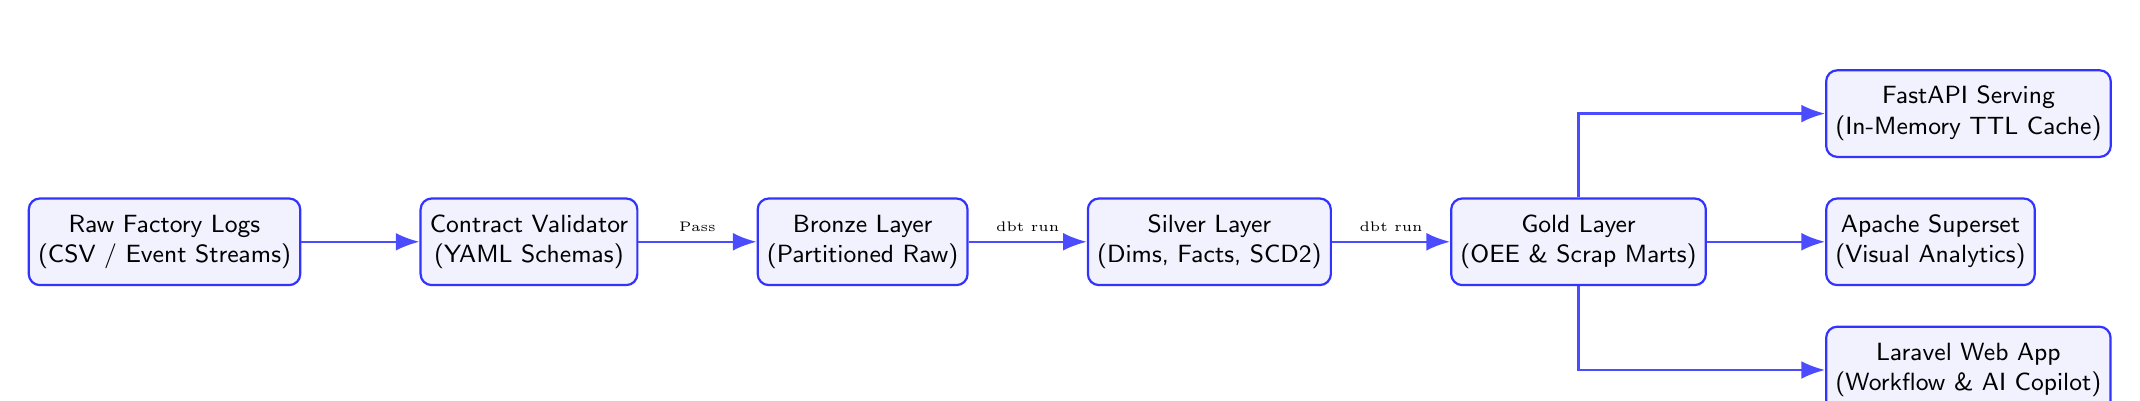
\begin{tikzpicture}[
    node distance=1.2cm and 1.5cm,
    box/.style={draw=blue!80, fill=blue!5, thick, rounded corners, minimum width=2.5cm, minimum height=1.1cm, align=center, font=\small\sffamily},
    arrow/.style={-{Latex[length=3mm]}, thick, draw=blue!70}
]

% Source
\node[box] (source) {Raw Factory Logs\\(CSV / Event Streams)};

% Ingestion & Governance
\node[box, right=of source] (contracts) {Contract Validator\\(YAML Schemas)};
\node[box, right=of contracts] (bronze) {Bronze Layer\\(Partitioned Raw)};

% Transformation
\node[box, right=of bronze] (silver) {Silver Layer\\(Dims, Facts, SCD2)};
\node[box, right=of silver] (gold) {Gold Layer\\(OEE \& Scrap Marts)};

% Serving & Apps
\node[box, above right=0.5cm and 1.5cm of gold] (fastapi) {FastAPI Serving\\(In-Memory TTL Cache)};
\node[box, right=1.5cm of gold] (superset) {Apache Superset\\(Visual Analytics)};
\node[box, below right=0.5cm and 1.5cm of gold] (laravel) {Laravel Web App\\(Workflow \& AI Copilot)};

% Arrows
\draw[arrow] (source) -- (contracts);
\draw[arrow] (contracts) -- node[above, font=\tiny]{Pass} (bronze);
\draw[arrow] (bronze) -- node[above, font=\tiny]{dbt run} (silver);
\draw[arrow] (silver) -- node[above, font=\tiny]{dbt run} (gold);
\draw[arrow] (gold) |- (fastapi);
\draw[arrow] (gold) -- (superset);
\draw[arrow] (gold) |- (laravel);

\end{tikzpicture}
\caption{FPLIP high-level architecture diagram detailing the data pipeline from raw logs to operational applications.}
\label{fig:high_level_arch}
\end{figure}

\begin{figure}[htbp]
\centering
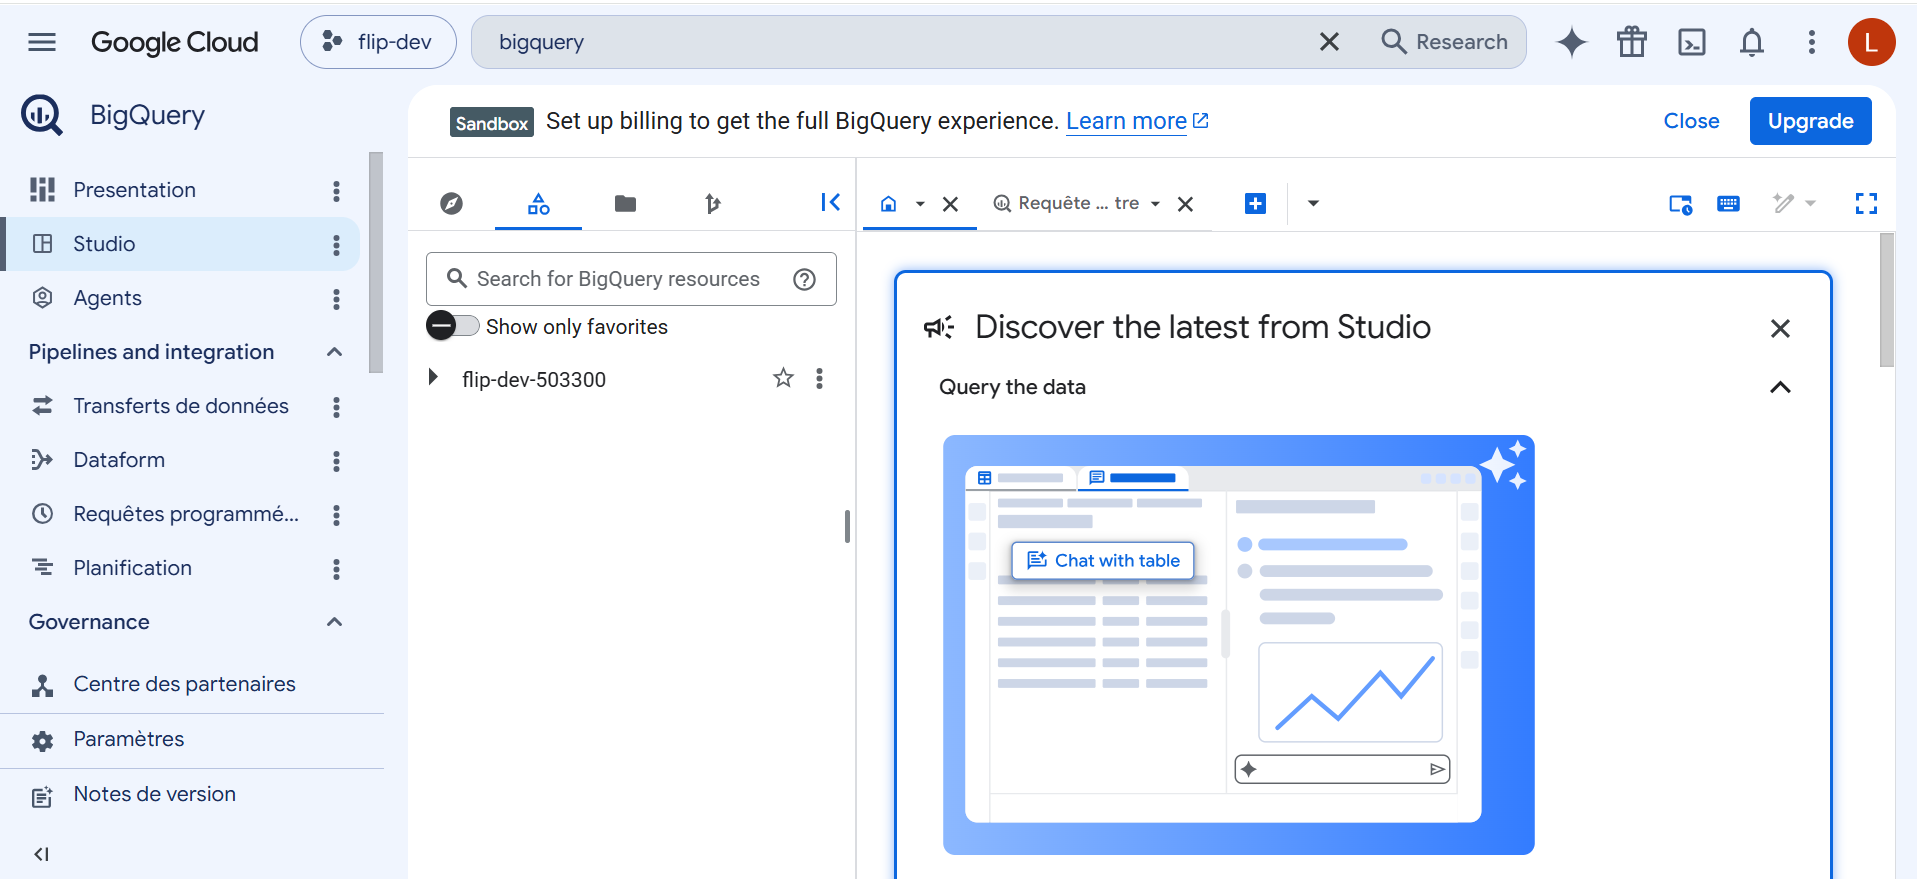
\includegraphics[width=0.95\textwidth]{bq_sandbox_active.png}
\caption{GCP BigQuery Sandbox active project workspace verifying zero-cost cloud deployment and isolated dataset setup.}
\label{fig:bq_sandbox_active}
\end{figure}

\begin{figure}[htbp]
\centering
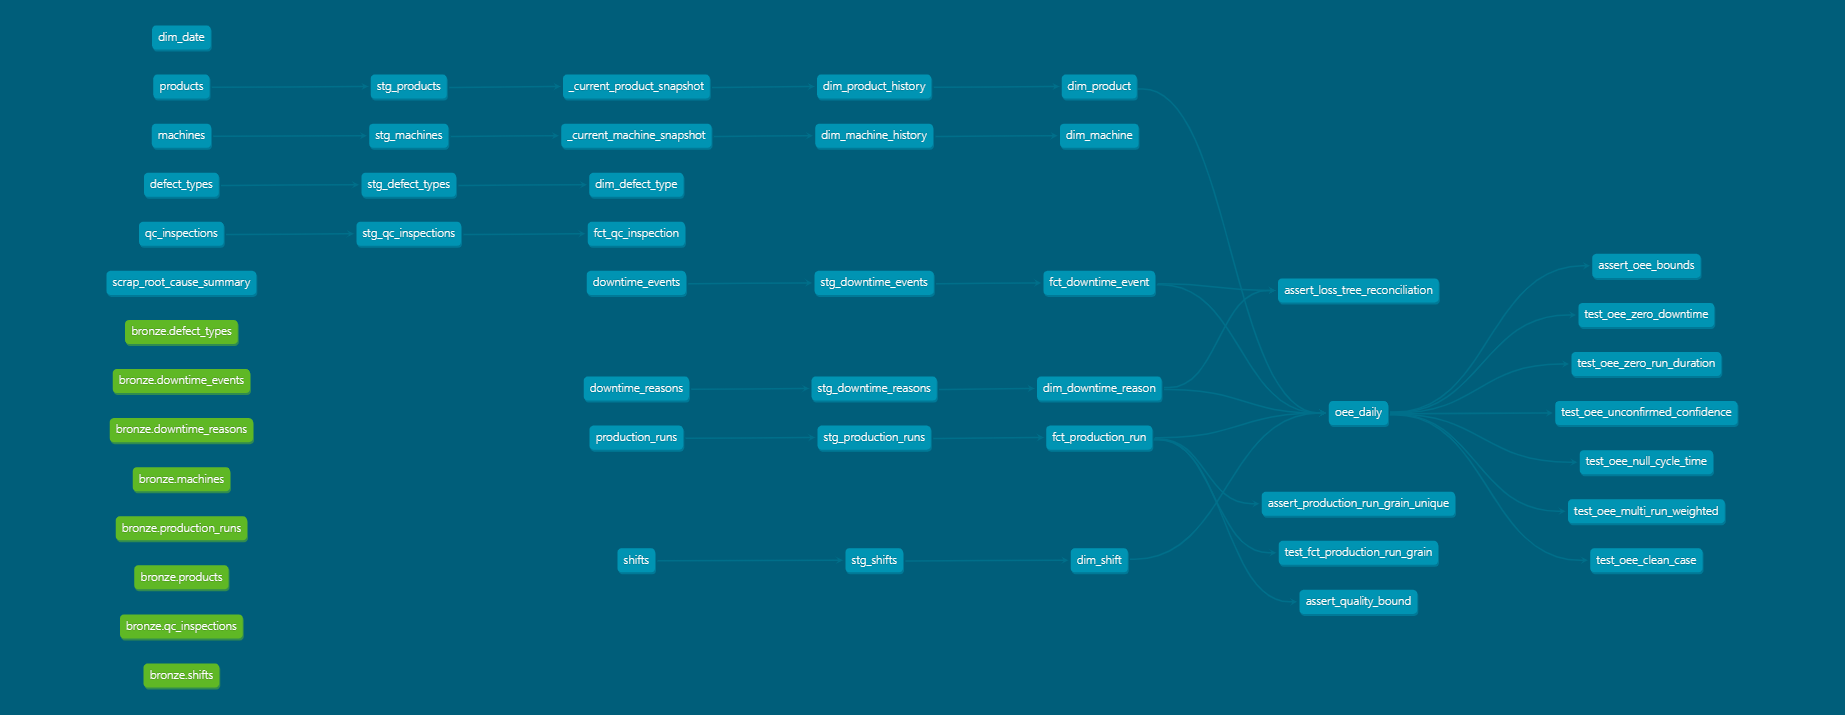
\includegraphics[width=0.95\textwidth]{lineage_graph_week5.png}
\caption{Automated dbt Medallion Lineage Graph displaying Bronze staging views, Silver dimensions/facts, and Gold OEE data marts.}
\label{fig:lineage_graph}
\end{figure}

\section{Technology Stack and Decision Rationale}
Every component in the FPLIP stack was selected based on strict architectural trade-offs, emphasizing zero cost, testability, enterprise patterns, and low operational overhead. Table~\ref{tab:tech_stack} summarizes the technology choices and their rationale.

\begin{table}[htbp]
\centering
\caption{FPLIP Technology Stack and Architectural Rationale}
\label{tab:tech_stack}
\begin{tabularx}{\textwidth}{l l X}
\toprule
\textbf{Layer / Component} & \textbf{Technology Selected} & \textbf{Architectural Rationale \& Decision} \\
\midrule
Cloud Warehouse & GCP BigQuery Sandbox & Zero financial cost, zero billing requirement, serverless SQL engine with 10\,GB storage. \\
Data Transformation & dbt (dbt-core / dbt-bigquery) & Declarative SQL modeling, version-controlled transformations, built-in testing framework. \\
Orchestration & Apache Airflow \& GitHub Actions & Airflow handles dependency DAGs; GitHub Actions provides free scheduled triggers without persistent VMs. \\
Serving API & FastAPI (Python 3.10) & Lightweight, async performance, strict Pydantic type validation, interactive OpenAPI docs. \\
Operational Web App & Laravel (PHP 11) & Native RBAC, built-in database migrations, Eloquent ORM, robust session/audit trail handling. \\
Visual Analytics & Apache Superset & Open-source, SQL-native visualization engine with granular dashboard filtering capabilities. \\
Infrastructure as Code & Terraform & Declarative GCP dataset and IAM service account provision, fully reproducible across environments. \\
\bottomrule
\end{tabularx}
\end{table}

\section{ELT vs. Traditional ETL Design Choice}
FPLIP implements a modern Extract-Load-Transform (ELT) pattern rather than traditional Extract-Transform-Load (ETL). In traditional ETL, transformations occur in an external processing server (e.g., Informatica, Talend) prior to warehouse loading. In FPLIP, raw factory data is validated against data contracts and loaded directly into the BigQuery Sandbox Bronze layer. 

All heavy transformations, dimensional modeling, and metric rollups take place inside BigQuery using dbt. This ELT strategy maximizes compute efficiency by leveraging BigQuery's distributed SQL engine, preserves raw historical data for future audits, and simplifies debugging by decoupling ingestion failures from transformation logic.

\section{Separation of Serving Concerns}
A core architectural feature of FPLIP is the deliberate decoupling of downstream consumers into three distinct, non-interfering interfaces:
\begin{enumerate}
    \item \textbf{FastAPI Serving Tier}: Serves external microservices and programmatic API clients requiring cached, low-latency JSON responses.
    \item \textbf{Apache Superset}: Serves executive managers and industrial engineers requiring interactive visual exploration, trends, and storytelling dashboards.
    \item \textbf{Laravel Web Application}: Serves operational staff (technicians and plant supervisors) requiring transactional workflows, task assignment, and grounded AI assistance.
\end{enumerate}
All three applications consume from the unified Gold data marts, ensuring a single source of truth across executive, operational, and algorithmic domains.


% --- CHAPTER 4: DATA PIPELINE IMPLEMENTATION ---
\chapter{Data Pipeline Implementation}
\label{chap:data_pipeline}

\section{Bronze Layer: Raw Ingestion and Data Contracts}
The Bronze layer acts as the raw landing zone for factory operational data. It consists of 8 raw event tables (\texttt{production\_runs}, \texttt{downtime\_events}, \texttt{qc\_inspections}) and 5 master reference tables (\texttt{machines}, \texttt{products}, \texttt{shifts}, \texttt{downtime\_reasons}, \texttt{defect\_types}).

\subsection{Pre-Ingestion Data Contracts}
Before data lands in BigQuery, FPLIP enforces shift-left data quality via YAML data contracts. Ingestion scripts parse incoming CSV files against predefined contract specifications. If a file contains invalid column types, missing required fields, or out-of-range numeric values, validation fails immediately, preventing corrupted data from entering Bronze. Listing~\ref{lst:yaml_contract} shows an excerpt of the quality control inspection contract, and Figure~\ref{fig:contract_validation} illustrates the contract validator execution.

\begin{figure}[htbp]
\centering
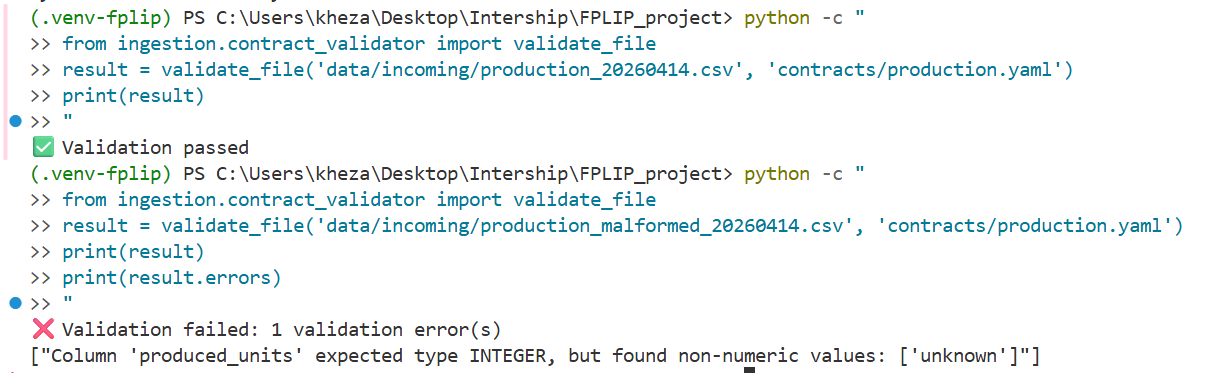
\includegraphics[width=0.85\textwidth]{contract_validator.png}
\caption{Shift-left YAML data contract pre-ingestion validation output verifying non-null, type, and value range integrity.}
\label{fig:contract_validation}
\end{figure}

\begin{lstlisting}[style=yamlstyle, caption={YAML Data Contract for Quality Control Inspections (\texttt{contracts/qc.yaml})}, label={lst:yaml_contract}]
version: 1
name: qc_inspections
columns:
  - name: inspection_id
    type: string
    required: true
  - name: machine_id
    type: string
    required: true
  - name: inspection_date
    type: date
    required: true
  - name: units_inspected
    type: integer
    required: true
    min_value: 1
  - name: units_rejected
    type: integer
    required: true
    min_value: 0
\end{lstlisting}

\subsection{Idempotent Load Pattern}
To guarantee idempotent ingestion within the BigQuery Sandbox, FPLIP uses partition-decorator targeting combined with BigQuery's \texttt{WRITE\_TRUNCATE} job disposition. Ingestion tasks target exact daily partitions (e.g., \texttt{production\_runs\$20260819}). Re-running an ingestion DAG for a given date completely replaces that specific partition without affecting historical partitions or duplicating records. Figure~\ref{fig:partitioned_tables} shows the resulting partitioned table layout in BigQuery, and Listing~\ref{lst:bronze_loader} details the loader execution snippet.

\begin{figure}[htbp]
\centering
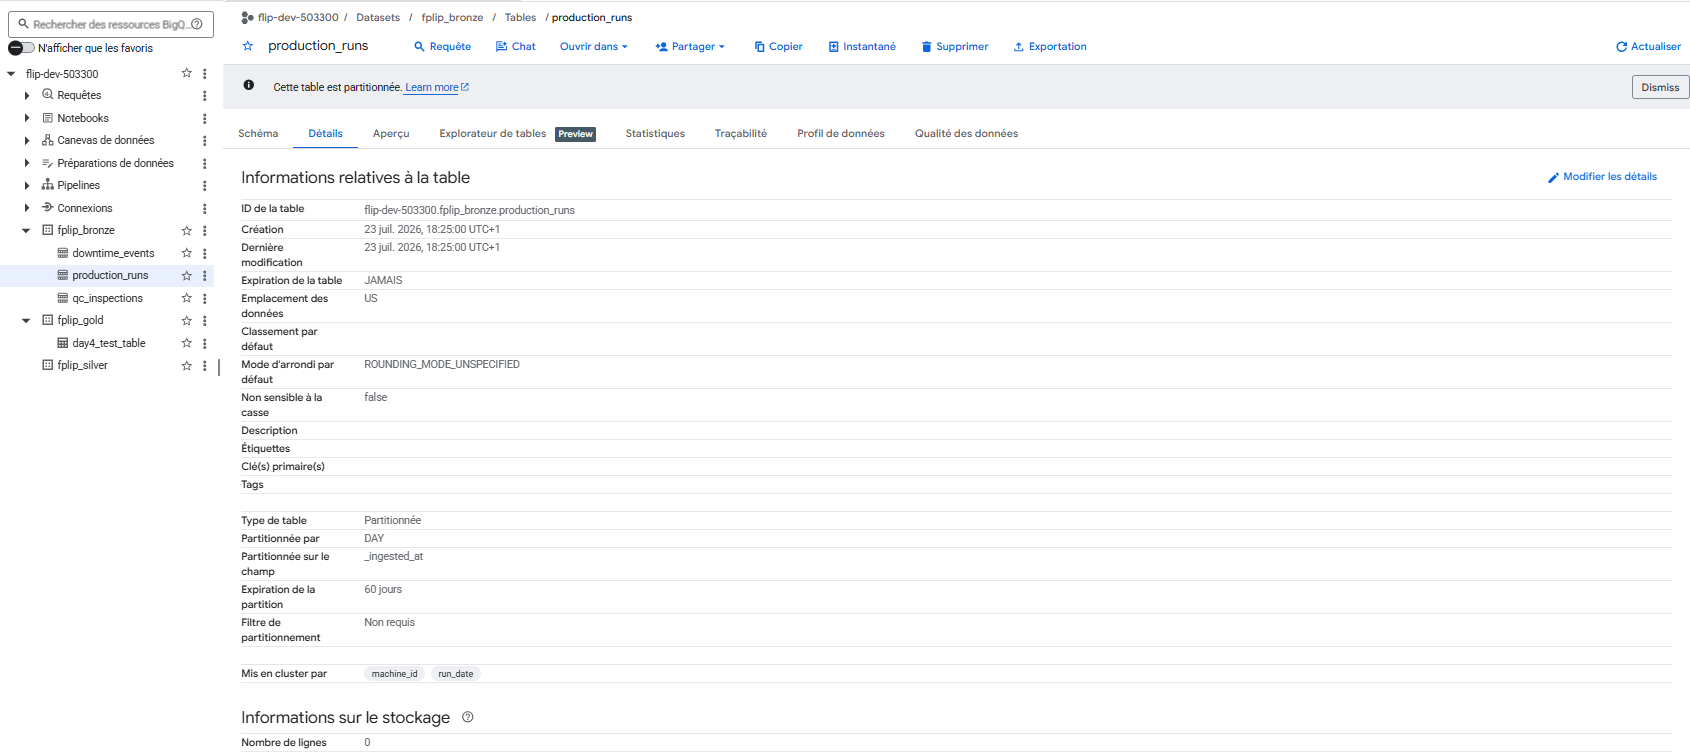
\includegraphics[width=0.95\textwidth]{week2_day3_partitioned_table.png}
\caption{BigQuery Sandbox table partition details displaying daily \texttt{\_ingested\_at} partition decorators and clustering.}
\label{fig:partitioned_tables}
\end{figure}

\begin{lstlisting}[style=pythonstyle, caption={Idempotent Partition Load Implementation (\texttt{ingestion/bronze\_loader.py})}, label={lst:bronze_loader}]
def load_to_bronze(df: pd.DataFrame, table_name: str, target_date: date, file_name: str) -> int:
    client = bigquery.Client(project=resolve_project_id())
    partition_str = target_date.strftime("%Y%m%d")
    destination = f"{resolve_project_id()}.fplip_bronze.{table_name}${partition_str}"
    
    job_config = bigquery.LoadJobConfig(
        write_disposition=bigquery.WriteDisposition.WRITE_TRUNCATE,
        source_format=bigquery.SourceFormat.PARQUET,
    )
    load_job = client.load_table_from_dataframe(df, destination, job_config=job_config)
    load_job.result(timeout=120)
    return len(df)
\end{lstlisting}

\section{Silver Layer: Cleaning, Dimensionality, and Hand-Rolled SCD2}
The Silver layer cleans raw Bronze records, establishes dimensional models, and tracks historical changes. Figure~\ref{fig:dbt_transform_run} illustrates the dbt transformation execution.

\begin{figure}[htbp]
\centering
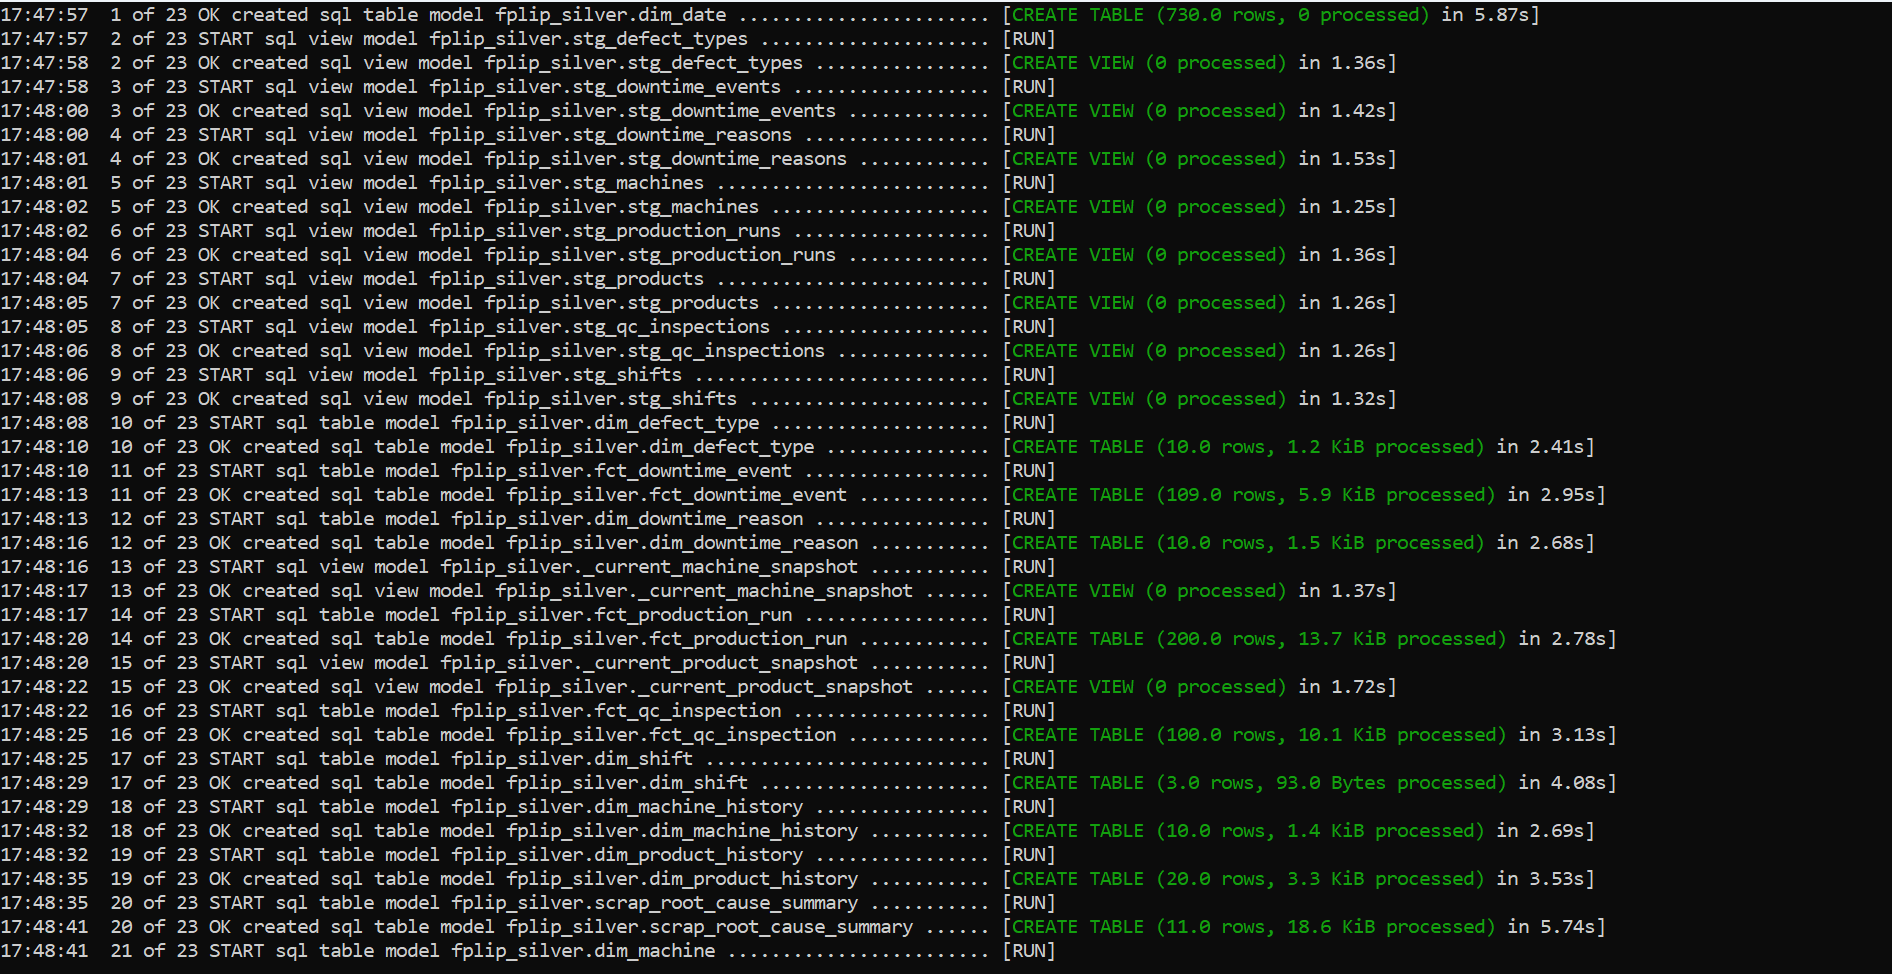
\includegraphics[width=0.95\textwidth]{05_dbt_silver_gold_models_execution.png}
\caption{dbt execution log building Silver staging views, dimensions, fact tables, and Gold OEE analytical marts.}
\label{fig:dbt_transform_run}
\end{figure}

\subsection{Staging Views and Dimensional Modeling}
Silver starts with 8 staging models (\texttt{stg\_*}) that apply lightweight data type casting and column renaming. From these staging assets, FPLIP constructs 6 dimension tables and 3 core fact tables:
\begin{itemize}
    \item \textbf{Dimensions}: \texttt{dim\_machine}, \texttt{dim\_product}, \texttt{dim\_shift}, \texttt{dim\_defect\_type}, \texttt{dim\_downtime\_reason}, \texttt{dim\_date}.
    \item \textbf{Facts}: \texttt{fct\_production\_run}, \texttt{fct\_downtime\_event}, \texttt{fct\_qc\_inspection}.
\end{itemize}

The explicit grain of \texttt{fct\_production\_run} is strictly defined as:
\begin{equation}
    \text{Grain: } (\text{machine\_id}, \text{shift\_id}, \text{product\_id}, \text{run\_date}, \text{run\_sequence\_number})
\end{equation}

\subsection{Hand-Rolled SCD Type 2 Without MERGE}
Because the GCP BigQuery Sandbox restricts DML \texttt{MERGE} statements, standard dbt SCD Type 2 snapshots cannot execute directly. FPLIP solves this via a hand-rolled DDL pattern using \texttt{CREATE OR REPLACE TABLE}. The query computes effective timestamps and active status flags using analytic window functions (\texttt{LEAD}), creating an immutable historical record without triggering blocked DML updates. Listing~\ref{lst:scd2_ddl} illustrates the pattern for \texttt{dim\_machine}.

\begin{lstlisting}[style=sqlstyle, caption={Hand-Rolled SCD2 DDL Pattern for \texttt{dim\_machine}}, label={lst:scd2_ddl}]
CREATE OR REPLACE TABLE `fplip-demo.fplip_silver.dim_machine` AS
WITH ranked_history AS (
  SELECT
    machine_id, machine_name, line_id, rated_speed_ppm, status,
    updated_at AS effective_date,
    LEAD(updated_at) OVER (PARTITION BY machine_id ORDER BY updated_at) AS raw_end_date
  FROM `fplip-demo.fplip_bronze.stg_machines`
)
SELECT
  GENERATE_UUID() AS machine_key,
  machine_id, machine_name, line_id, rated_speed_ppm, status,
  effective_date,
  COALESCE(raw_end_date, TIMESTAMP('2099-12-31 23:59:59')) AS end_date,
  CASE WHEN raw_end_date IS NULL THEN TRUE ELSE FALSE END AS is_current
FROM ranked_history;
\end{lstlisting}

\subsection{Silver Testing Taxonomies}
Schema testing on Silver assets includes \texttt{not\_null}, \texttt{unique}, and \texttt{accepted\_values}. Foreign key integrity is validated using \texttt{relationships} tests configured with \texttt{severity: warn} on nullable references, preventing non-critical QC logs from failing the pipeline while surfacing data quality alerts.

\section{Gold Layer: Aggregated Analytical Marts}
The Gold layer provides curated, business-ready data marts optimized for OEE computation and scrap root-cause analysis.

\subsection{OEE Computation and Loss Attribution (\texttt{oee\_daily})}
The \texttt{oee\_daily} table computes daily operational metrics per machine and shift. Availability is calculated at the shift level using total planned production time and downtime events. Performance and Quality are computed at the individual run level and aggregated upward. Listing~\ref{lst:oee_gold} demonstrates the SQL transformation logic for \texttt{oee\_daily}.

\begin{lstlisting}[style=sqlstyle, caption={Gold Mart OEE and Loss Attribution Logic (\texttt{models/gold/oee\_daily.sql})}, label={lst:oee_gold}]
WITH shift_planned_time AS (
  SELECT machine_id, shift_id, run_date AS date_id,
         SUM(planned_units / NULLIF(rated_speed_ppm, 0) * 60) AS planned_time_sec
  FROM {{ ref('fct_production_run') }} JOIN {{ ref('dim_machine') }} USING (machine_id)
  GROUP BY 1, 2, 3
),
downtime_summary AS (
  SELECT machine_id, shift_id, DATE(start_time) AS date_id,
         SUM(duration_sec) AS total_downtime_sec
  FROM {{ ref('fct_downtime_event') }} GROUP BY 1, 2, 3
)
SELECT
  p.machine_id, p.shift_id, p.date_id,
  -- Component Calculations
  SAFE_DIVIDE(planned_time_sec - COALESCE(total_downtime_sec, 0), planned_time_sec) AS availability,
  SAFE_DIVIDE(total_produced_units, total_operating_time * rated_speed_ppm) AS performance,
  SAFE_DIVIDE(total_good_units, total_produced_units) AS quality,
  -- Overall OEE
  (availability * performance * quality) AS oee,
  -- Loss Attribution (Hours)
  (total_downtime_sec / 3600.0) AS availability_loss_hours,
  ((total_operating_time - (total_produced_units / rated_speed_ppm)) / 3600.0) AS performance_loss_hours,
  (((total_produced_units - total_good_units) / rated_speed_ppm) / 3600.0) AS quality_loss_hours
FROM shift_planned_time p LEFT JOIN downtime_summary USING (machine_id, shift_id, date_id);
\end{lstlisting}

\subsection{Scrap Root-Cause Attribution (\texttt{scrap\_root\_cause\_summary})}
The \texttt{scrap\_root\_cause\_summary} table joins \texttt{fct\_qc\_inspection} with \texttt{fct\_production\_run} and \texttt{dim\_defect\_type} to categorize scrap by defect severity and root cause. To handle cases where a QC inspection record is missing an explicit production run reference, the model employs a fallback join on \texttt{(machine\_id, inspection\_date)}, ensuring metadata like \texttt{machine\_id}, \texttt{shift\_id}, and \texttt{product\_id} are preserved rather than defaulting to \texttt{'UNKNOWN'}.

\subsection{Gold Verification: Model Contracts and Singular Tests}
All Gold models enforce strict dbt model contracts (\texttt{contract: {enforced: true}}). Furthermore, three custom singular SQL tests protect data sanity:
\begin{enumerate}
    \item \texttt{assert\_oee\_bounds}: Asserts that Availability, Performance, Quality, and overall OEE remain between $0.0$ and $1.0$.
    \item \texttt{assert\_quality\_ceiling}: Asserts that \texttt{good\_units} never exceeds \texttt{produced\_units}.
    \item \texttt{assert\_loss\_reconciliation}: Asserts that total available shift time equals Operating Time + Availability Loss + Performance Loss + Quality Loss within a $0.1\%$ tolerance margin.
\end{enumerate}

Figure~\ref{fig:dbt_test_suite} demonstrates the complete execution of the 85-test suite across Silver and Gold models.

\begin{figure}[htbp]
\centering
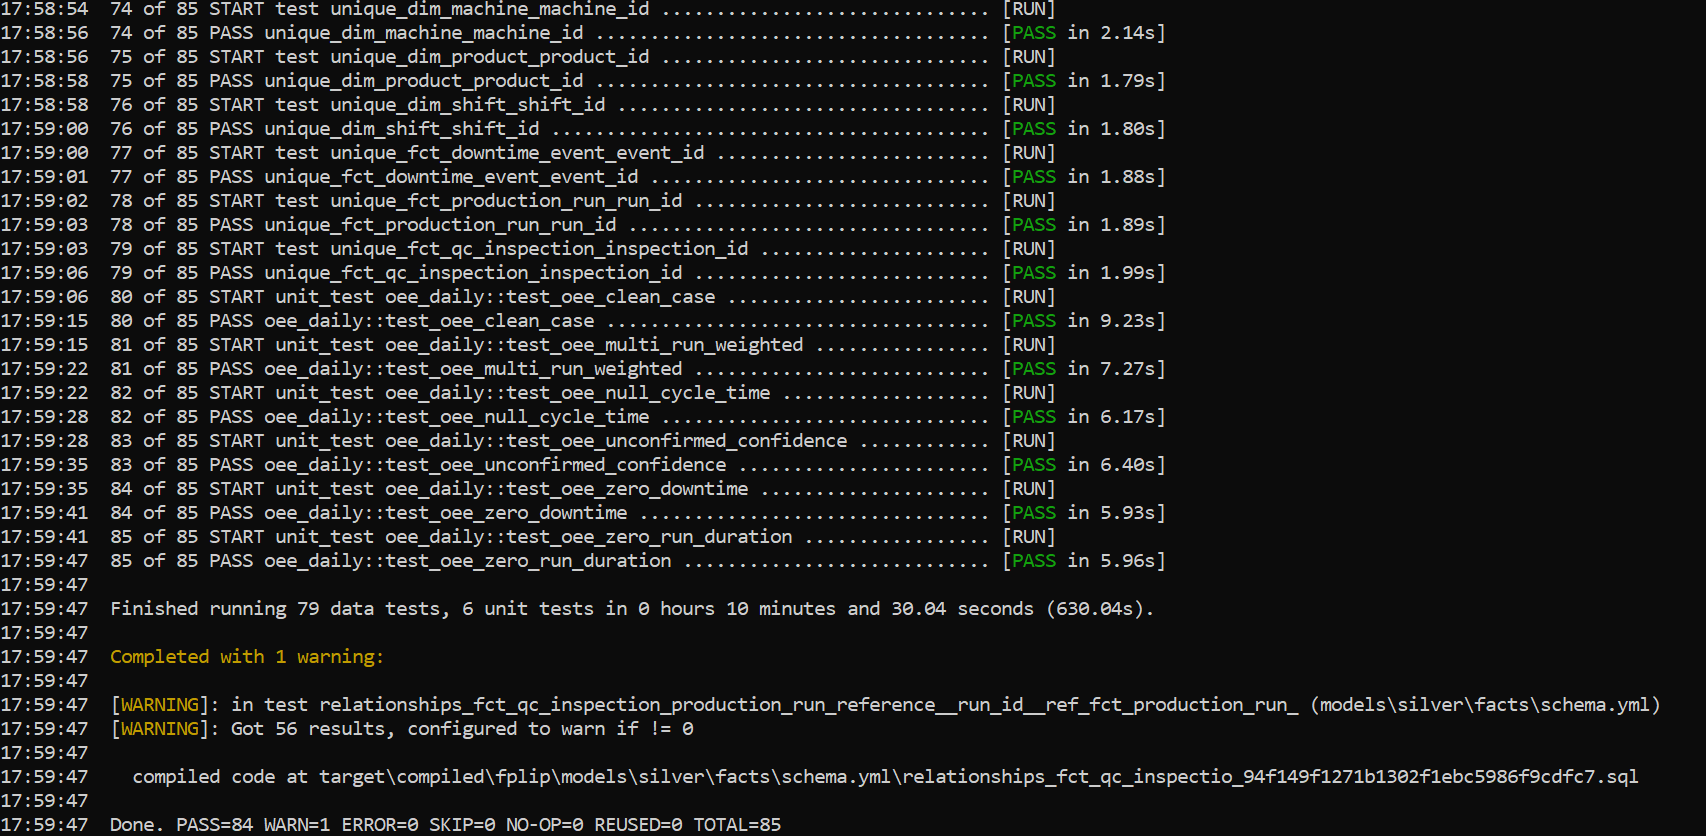
\includegraphics[width=0.95\textwidth]{07_dbt_test_suite_execution.png}
\caption{dbt test suite execution verifying 85 assertions across generic schema tests, singular domain invariants, and unit tests.}
\label{fig:dbt_test_suite}
\end{figure}


% --- CHAPTER 5: ORCHESTRATION & AUTOMATION ---
\chapter{Orchestration \& Automation}
\label{chap:orchestration}

\section{Airflow Orchestration DAGs}
FPLIP orchestrates data flows across three modular Apache Airflow DAGs:
\begin{enumerate}
    \item \texttt{ingestion\_dag}: Runs parallel extraction and contract validation tasks for production, downtime, and QC logs.
    \item \texttt{dbt\_transform\_dag}: Triggers Silver dimension/fact builds and Gold analytical mart transformations sequentially.
    \item \texttt{data\_quality\_dag}: Executes dbt test suites, singular tests, and sends Slack status notifications.
\end{enumerate}

Figure~\ref{fig:airflow_dags} illustrates the Apache Airflow Web UI DAG management interface.

\begin{figure}[htbp]
\centering
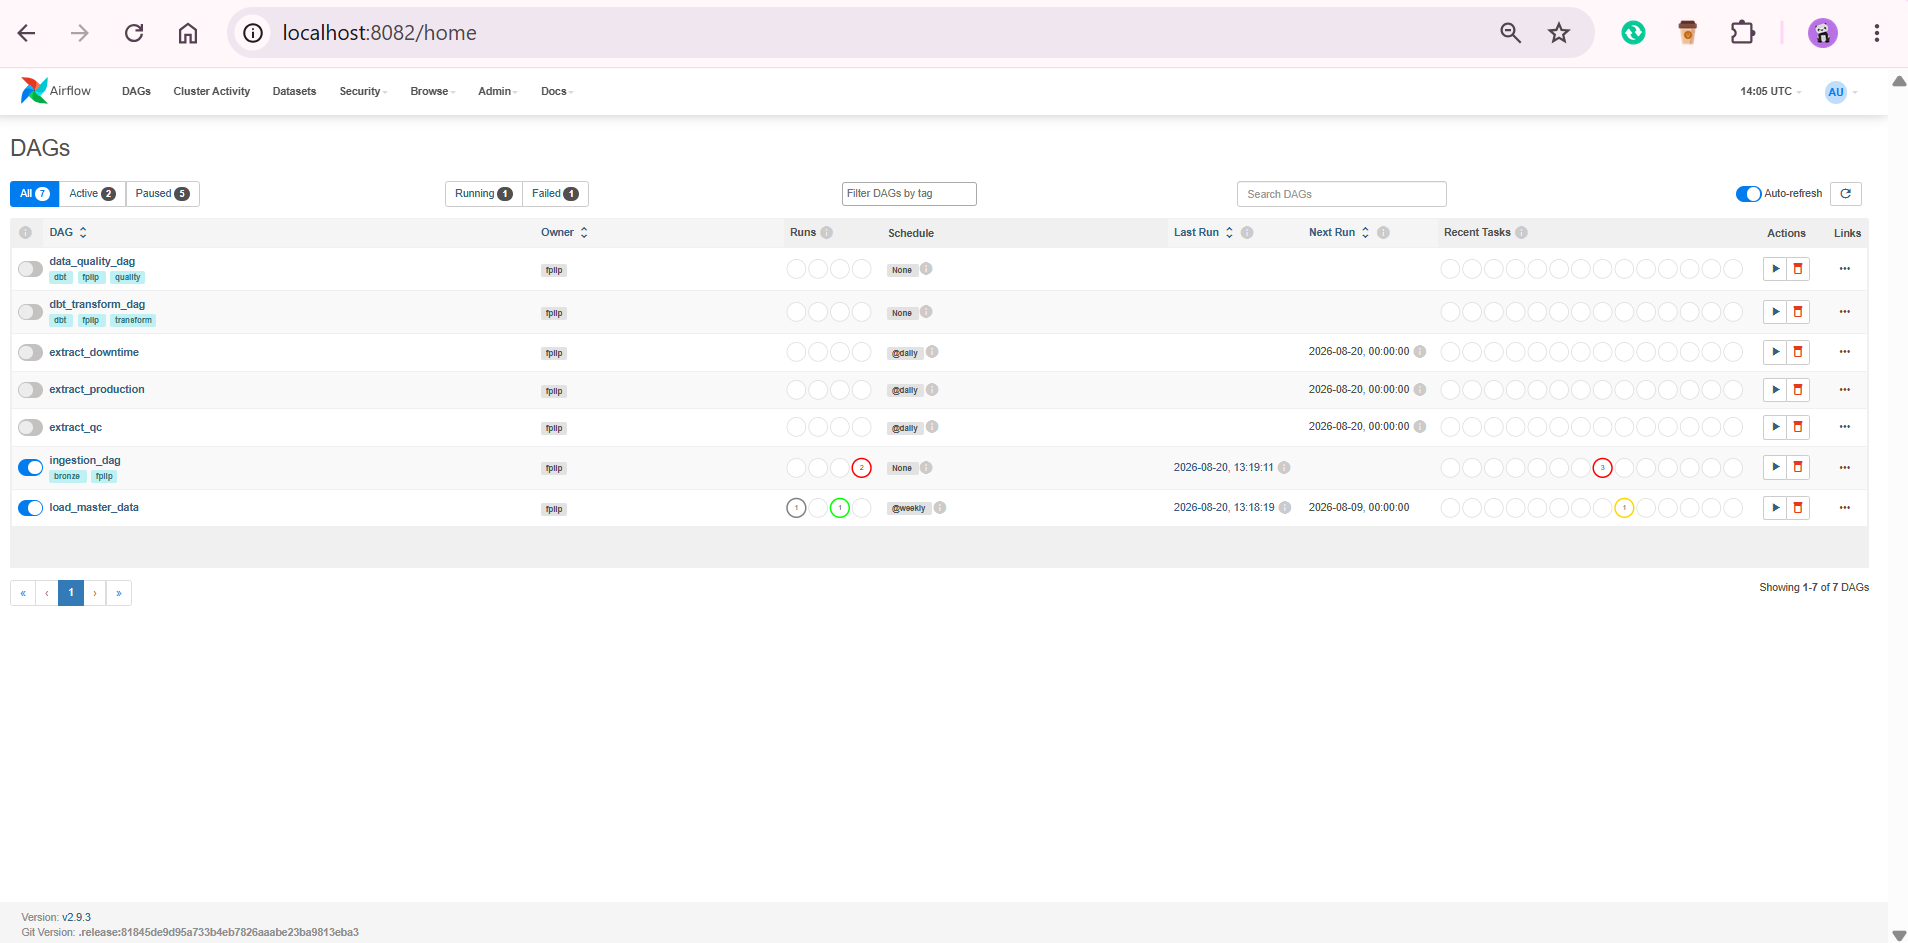
\includegraphics[width=0.95\textwidth]{13_airflow_dags_overview.png}
\caption{Apache Airflow Web UI DAG Overview displaying active orchestration DAGs (\texttt{ingestion\_dag}, \texttt{dbt\_transform\_dag}, \texttt{data\_quality\_dag}).}
\label{fig:airflow_dags}
\end{figure}

To ensure seamless local and container execution, Airflow tasks invoke dynamic Python path resolvers to locate the container's dedicated virtual environment (\texttt{/opt/airflow/.venv-fplip/bin/dbt}).

\section{Pipeline Script Chaining (\texttt{run\_pipeline.sh})}
End-to-end execution can be triggered via a unified CLI entrypoint (\texttt{run\_pipeline.sh}). The script automates contract validation, Bronze partition loads, dbt model transformations, and dbt test execution in sequence, returning an exit code of \texttt{0} only if all stages pass.

\section{Slack Alerting and Operational Callbacks}
Airflow DAGs utilize on-failure callbacks (\texttt{on\_failure\_callback = notify\_failure}) to notify operations teams immediately if a pipeline task fails. Notifications post JSON payloads to a Slack webhook containing the DAG ID, failed task ID, execution date, and error stack trace excerpt.

\section{CI/CD Pipeline with Ephemeral Datasets}
Continuous Integration and Continuous Deployment (CI/CD) is implemented using GitHub Actions. The workflow runs on every Pull Request and consists of 5 parallel and sequential jobs:
\begin{enumerate}
    \item \textbf{Linting}: Python code linting via \texttt{flake8} and SQL formatting checks via \texttt{sqlfluff}.
    \item \textbf{Contract Check}: Executes contract validation tests against sample datasets.
    \item \textbf{Ephemeral dbt Test}: Provisions a unique, temporary GCP BigQuery dataset (e.g., \texttt{ci\_fplip\_pr\_42}), runs dbt models, executes dbt test suites, and teardowns the temporary dataset upon completion.
    \item \textbf{Terraform Plan}: Validates infrastructure files and generates execution plans.
    \item \textbf{Docker Build}: Validates container images for web app and API dependencies.
\end{enumerate}

Figure~\ref{fig:ci_workflow} shows the GitHub Actions execution verifying all 5 CI jobs.

\begin{figure}[htbp]
\centering
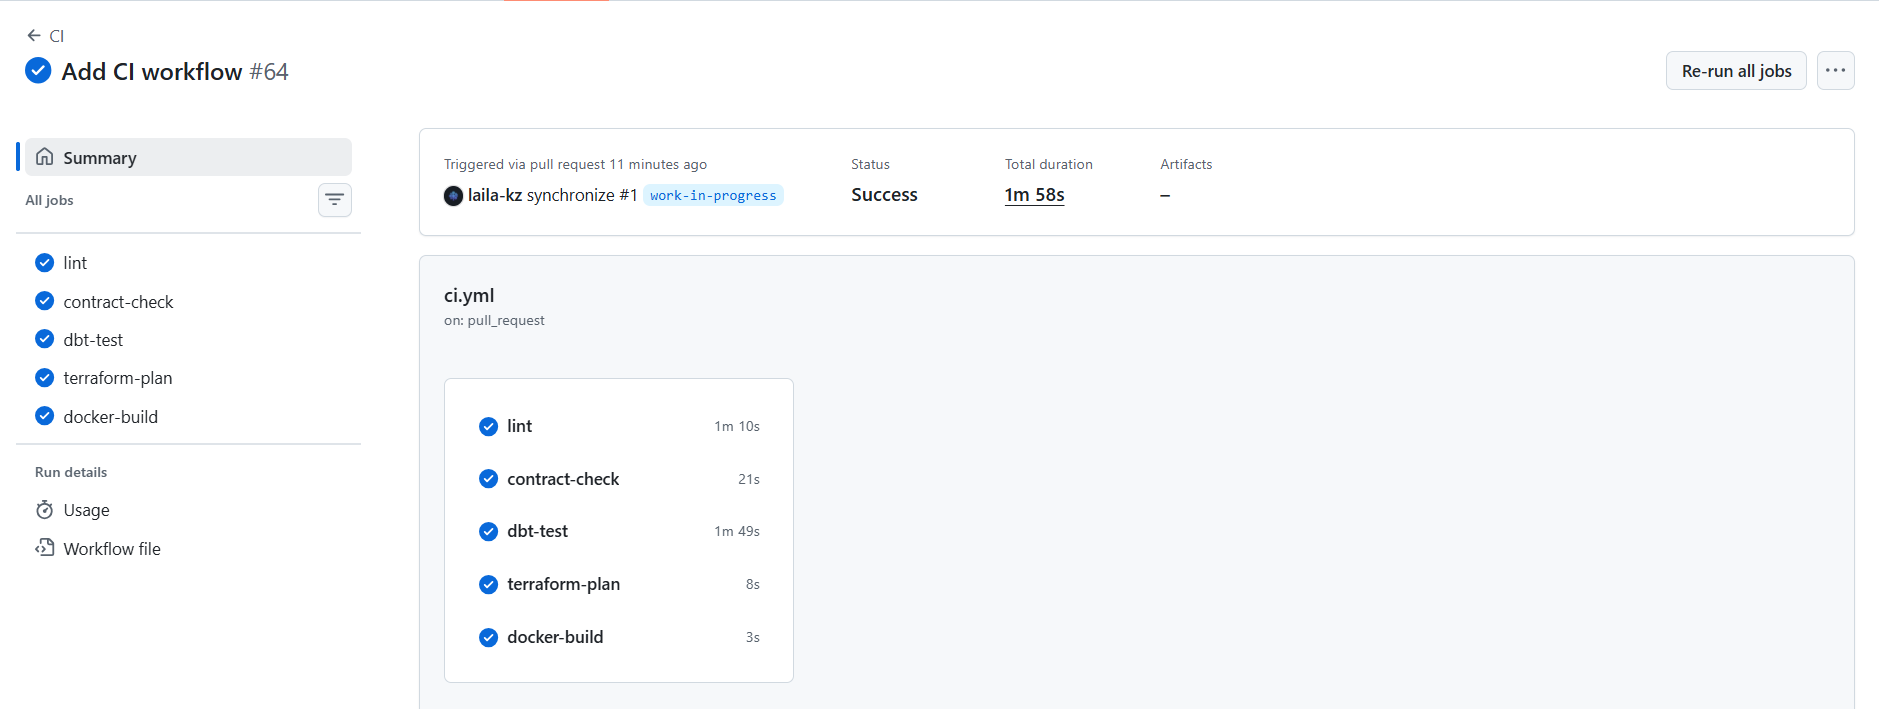
\includegraphics[width=0.95\textwidth]{ci_workflow_success.png}
\caption{GitHub Actions 5-job CI/CD workflow execution success with ephemeral per-PR BigQuery dataset isolation.}
\label{fig:ci_workflow}
\end{figure}


% --- CHAPTER 6: WEB APPLICATION ---
\chapter{Web Application (Laravel)}
\label{chap:web_application}

\section{Application Architecture and RBAC}
The FPLIP operational web application is built using Laravel (PHP 11). It provides plant personnel with real-time operational visibility and task execution capabilities. Access control is managed through native Role-Based Access Control (RBAC):
\begin{itemize}
    \item \textbf{Plant Manager}: Has full administrative privileges, configures shift thresholds, creates investigations, assigns maintenance tasks, and accesses scrap risk predictions.
    \item \textbf{Line Technician}: Accesses assigned maintenance tasks, updates repair statuses, logs machine fix logs, and closes resolved investigation tickets.
\end{itemize}

Figure~\ref{fig:laravel_login} displays the secure authentication portal for plant staff.

\begin{figure}[htbp]
\centering
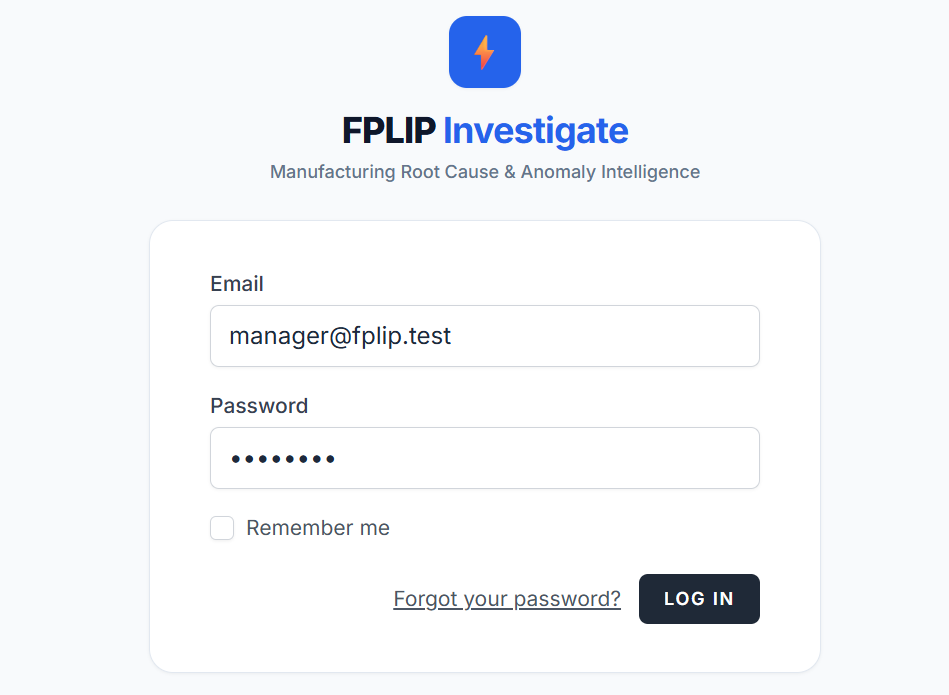
\includegraphics[width=0.8\textwidth]{15_laravel_investigate_login.png}
\caption{FPLIP Investigate operational web application secure login interface with Role-Based Access Control (RBAC).}
\label{fig:laravel_login}
\end{figure}

\section{Investigation Lifecycle Workflow}
The application operationalizes analytical signals through a 5-stage investigation lifecycle:
\begin{equation}
    \text{Detect} \longrightarrow \text{Investigate} \longrightarrow \text{Assign} \longrightarrow \text{Fix} \longrightarrow \text{Close}
\end{equation}

When the Gold layer detects an OEE dip below threshold ($<75\%$) or a scrap spike ($>5\%$), an automated signal triggers an investigation candidate. Managers review the event on the Plant Signal Intelligence Dashboard (Figure~\ref{fig:plant_signals_dash}) and review active anomaly cards (Figure~\ref{fig:active_plant_signals}).

\begin{figure}[htbp]
\centering
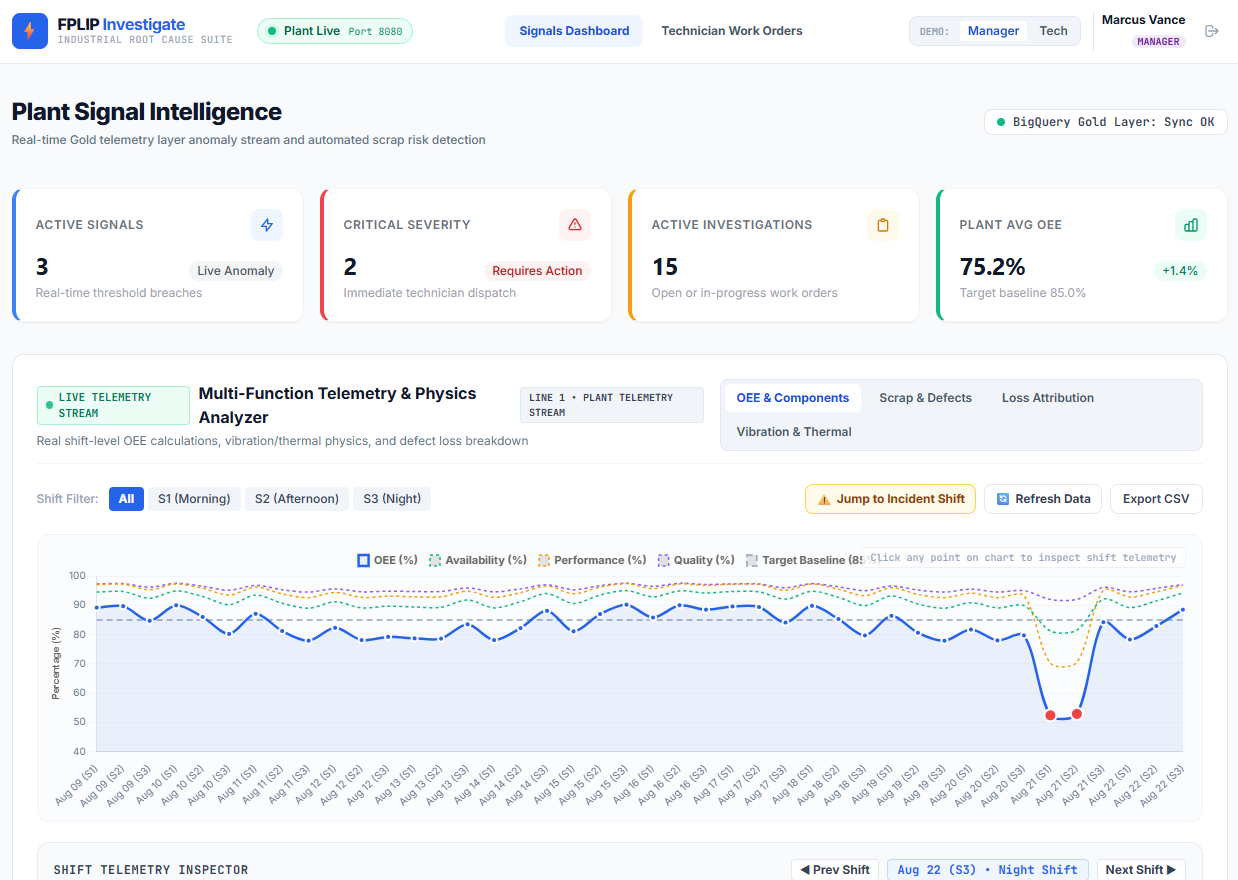
\includegraphics[width=0.95\textwidth]{16_plant_signal_intelligence_dashboard.png}
\caption{Plant Signal Intelligence Dashboard showing live shift telemetry streams, OEE component breakdowns, and active signal cards.}
\label{fig:plant_signals_dash}
\end{figure}

\begin{figure}[htbp]
\centering
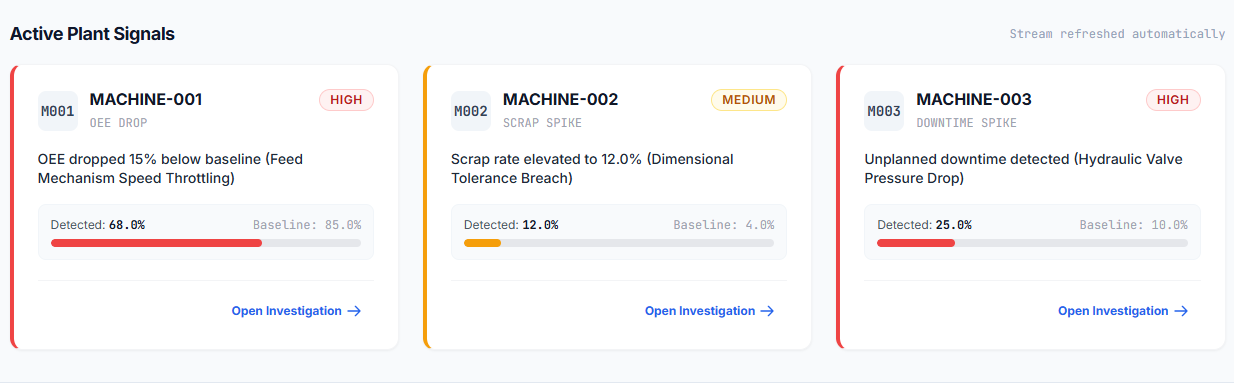
\includegraphics[width=0.95\textwidth]{17_active_plant_signals_cards.png}
\caption{Active Anomaly Signal Cards displaying real-time OEE drops, scrap spikes, and direct investigation dispatch triggers.}
\label{fig:active_plant_signals}
\end{figure}

\section{Audit Trail Governance}
To ensure industrial compliance and operational accountability, all user state changes (task updates, role adjustments, parameter modifications) are captured in an immutable \texttt{audit\_logs} table. Each audit log captures the \texttt{user\_id}, \texttt{action\_type}, \texttt{target\_entity}, timestamp, and pre/post-change JSON state payloads.

\section{ML Scrap Risk \& AI Copilot UI Integration}
The Laravel interface surfaces ML-driven scrap risk predictions on the active run dashboard. If a run's predicted scrap probability exceeds $0.65$, a visual warning indicator alerts the operator. Users can click the alert to activate the embedded AI Copilot drawer (Figure~\ref{fig:gemini_ai_diagnostic}), which returns grounded explanations explaining the primary risk drivers. Technicians submit physical root-cause findings and corrective actions using the dedicated work order form (Figure~\ref{fig:technician_work_order}).

\begin{figure}[htbp]
\centering
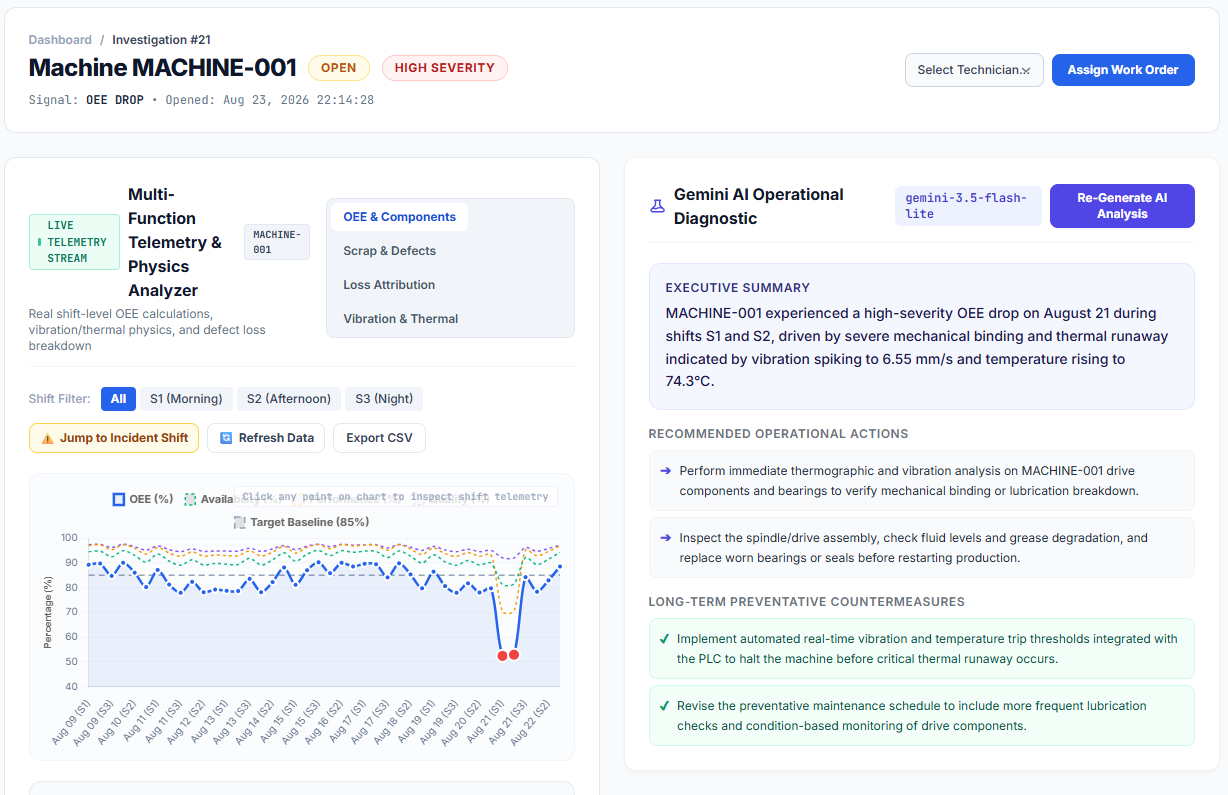
\includegraphics[width=0.95\textwidth]{18_gemini_ai_operational_diagnostic.png}
\caption{Grounded Gemini AI Operational Diagnostic drawer presenting executive summaries, recommended actions, and preventative countermeasures.}
\label{fig:gemini_ai_diagnostic}
\end{figure}

\begin{figure}[htbp]
\centering
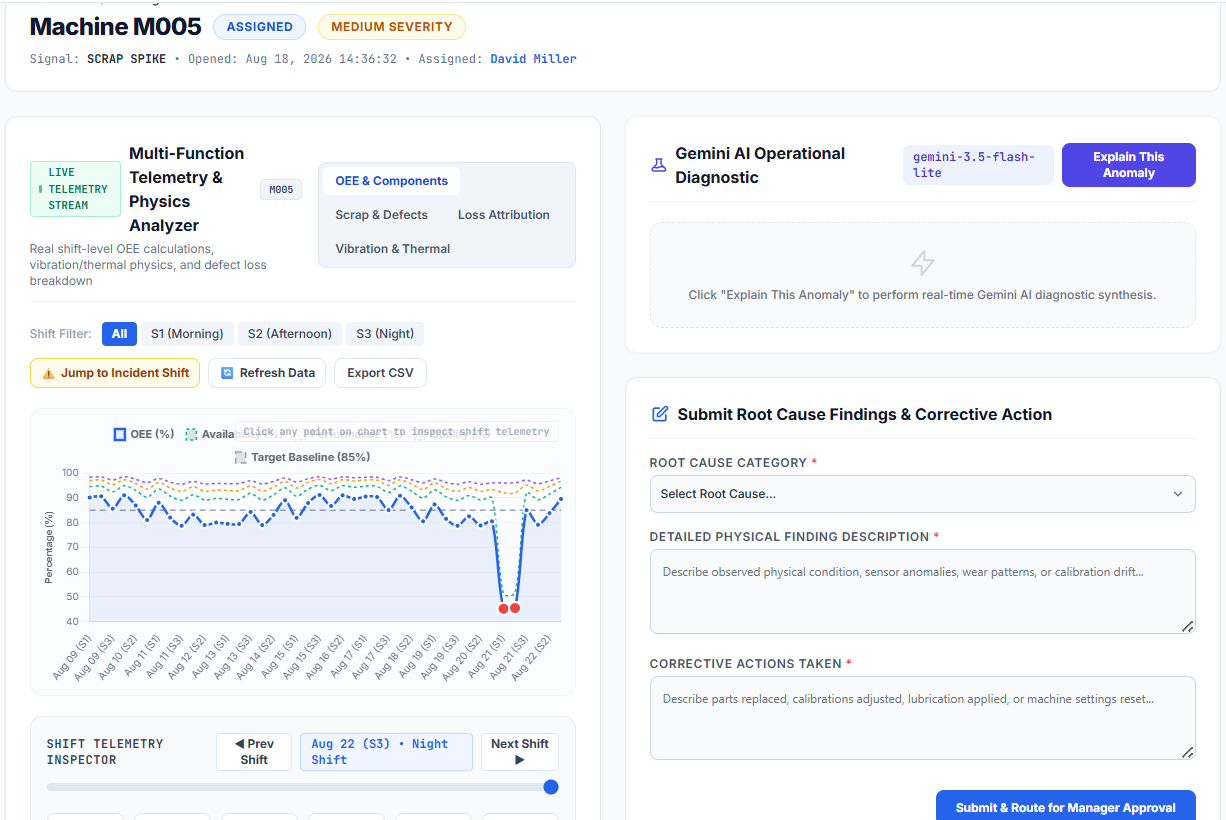
\includegraphics[width=0.95\textwidth]{19_technician_root_cause_submission_form.png}
\caption{Line Technician Root Cause Submission Form for submitting physical findings, corrective actions, and routing for manager approval.}
\label{fig:technician_work_order}
\end{figure}


% --- CHAPTER 7: DASHBOARD & VISUALIZATION ---
\chapter{Dashboard \& Visualization (Superset)}
\label{chap:dashboard}

\section{Apache Superset Architecture}
Apache Superset serves as the primary visual analytics layer for FPLIP. Connected directly to BigQuery Gold marts via SQLAlchemy, Superset provides real-time data exploration without requiring complex intermediate OLAP cubes.

\section{4-Row Storytelling Dashboard Layout}
The main executive dashboard is designed around an inverted pyramid storytelling layout, structured into 4 logical horizontal rows:
\begin{enumerate}
    \item \textbf{Row 1: Executive KPI Header}: Big Number KPI tiles displaying overall OEE, Total Produced Units, Total Scrap Units, and Average Quality Rate.
    \item \textbf{Row 2: Temporal Trends}: Line charts illustrating daily OEE trends and shift-by-shift performance comparisons.
    \item \textbf{Row 3: Dimensional Breakdown}: Bar charts displaying OEE across individual machines, product SKUs, and manufacturing lines.
    \item \textbf{Row 4: Loss Attribution \& Scrap Root-Cause}: Sunburst and stacked bar charts detailing Availability vs. Performance vs. Quality loss hours, alongside top defect categories.
\end{enumerate}

Figure~\ref{fig:superset_dashboard} illustrates the export of the Apache Superset executive dashboard.

\begin{figure}[htbp]
\centering
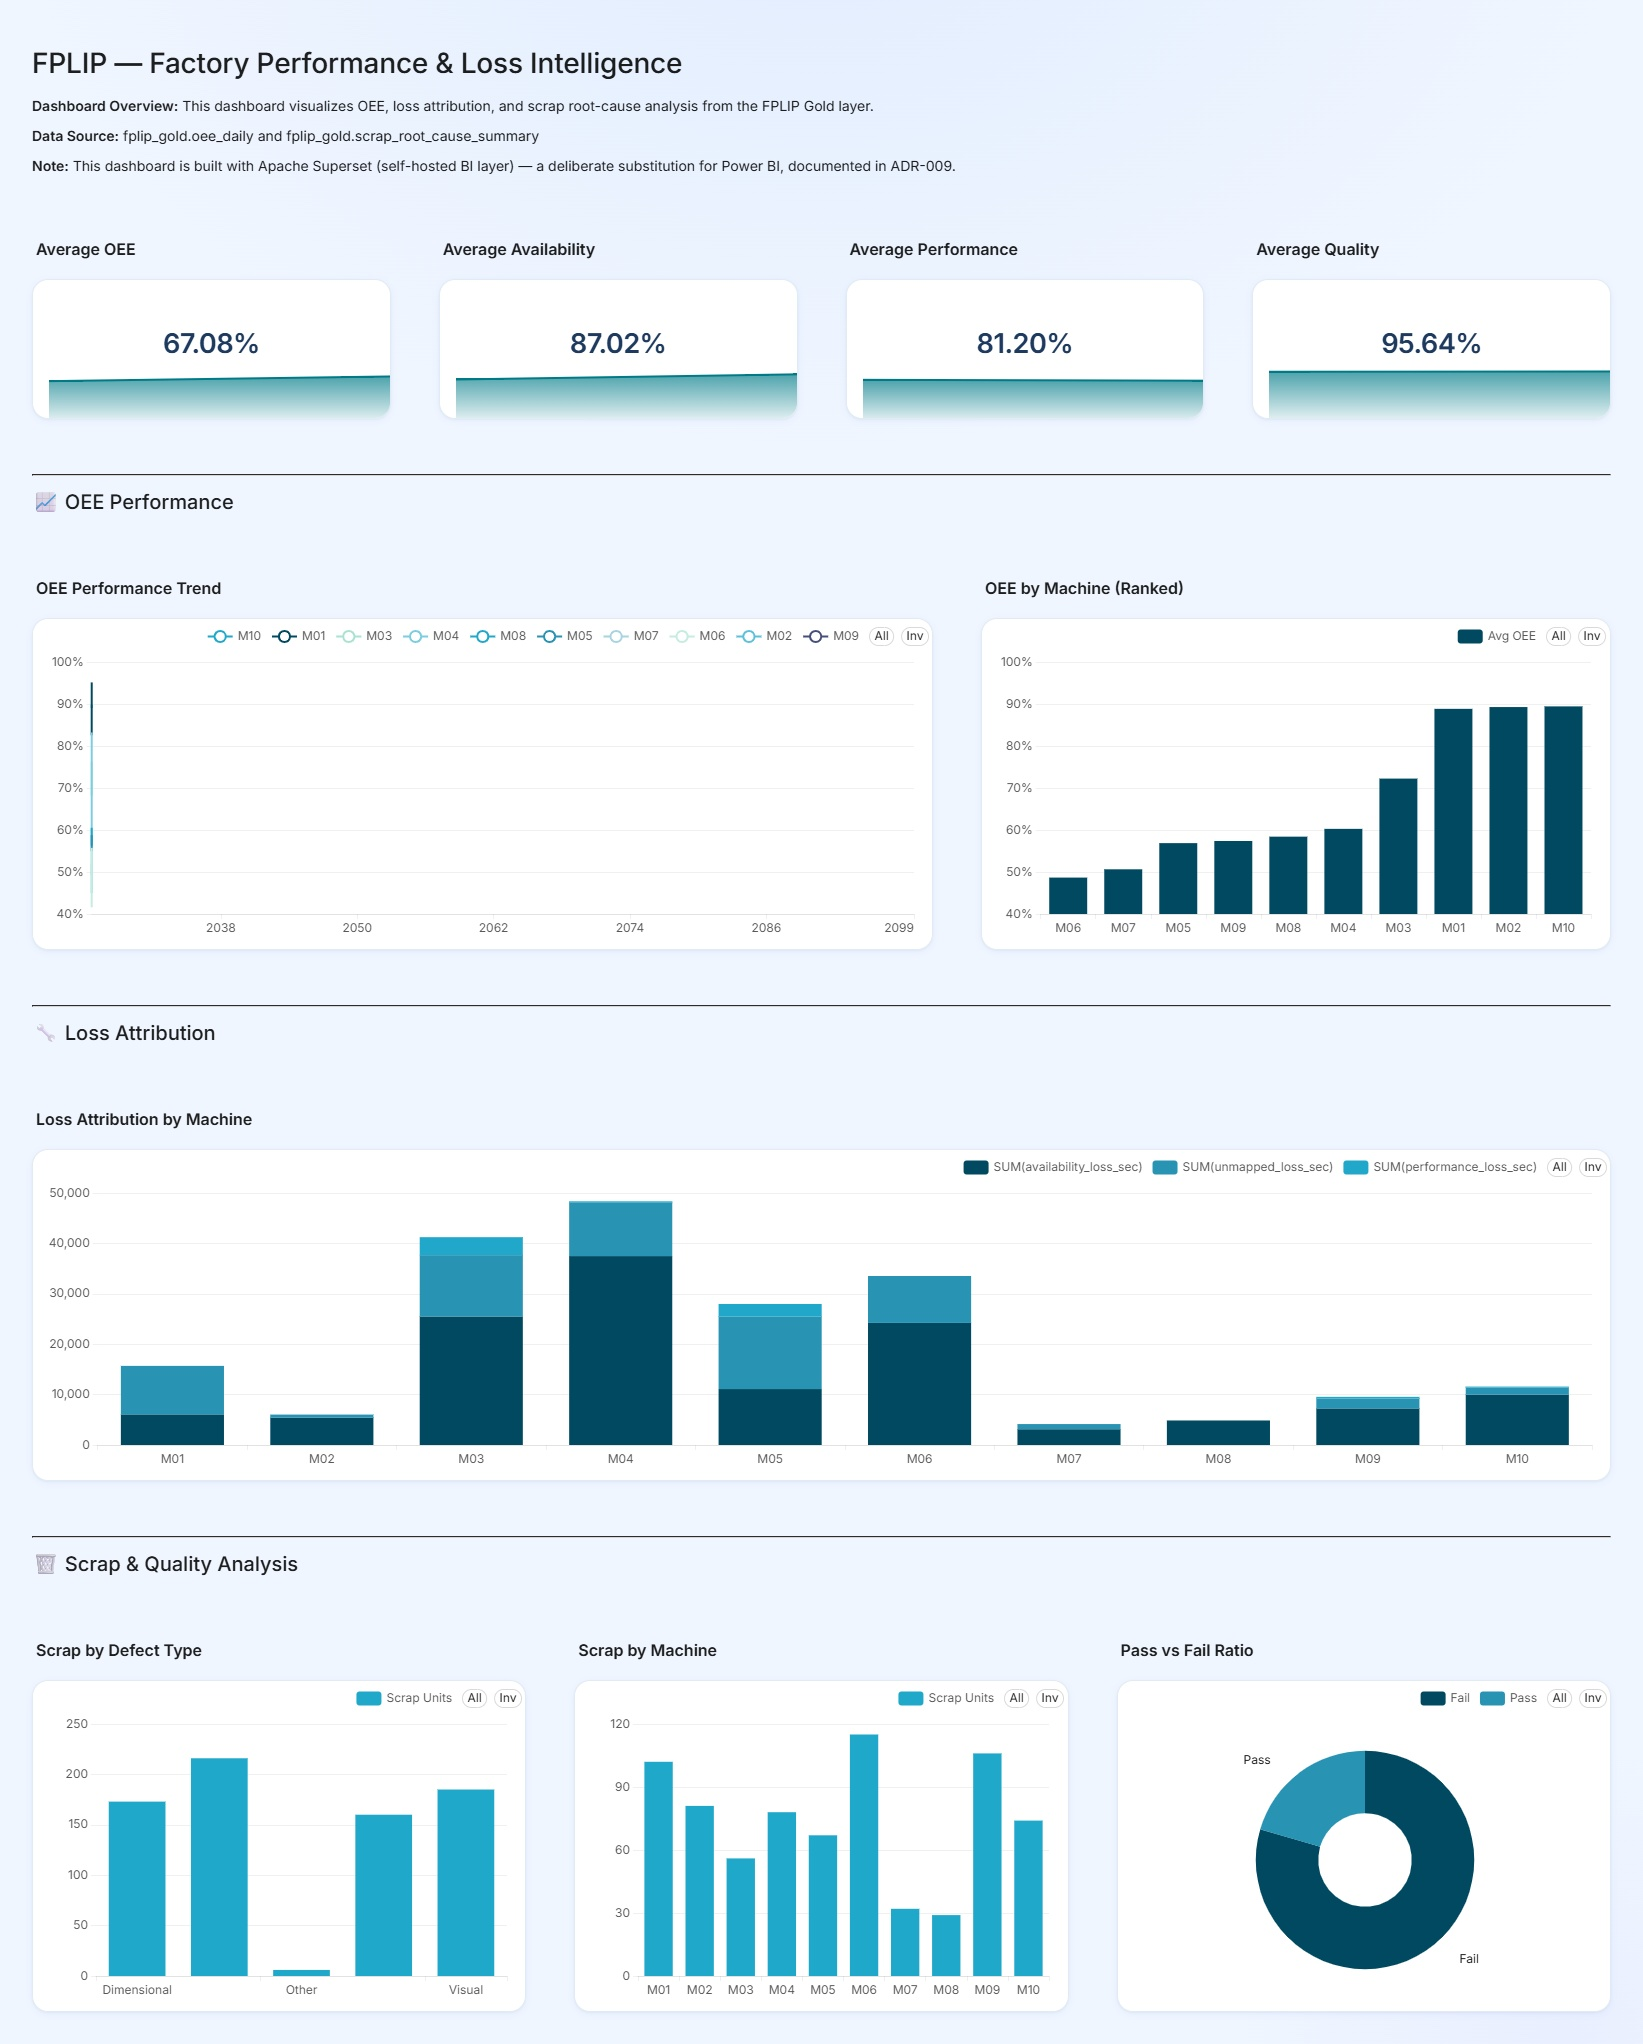
\includegraphics[width=0.95\textwidth]{superset_dashboard_export.jpg}
\caption{Apache Superset 4-Row Storytelling OEE \& Scrap Root Cause Analytics Dashboard.}
\label{fig:superset_dashboard}
\end{figure}

\section{Global Filters and TTL Caching Strategy}
Global dashboard filters allow users to filter all charts dynamically by date range, machine ID, and product category. To protect GCP BigQuery Sandbox query quotas, Superset is configured with a 4-hour in-memory TTL query cache. Repeated dashboard views serve cached data instantly, executing live BigQuery queries only when global filter parameters are modified.


% --- CHAPTER 8: ML & AI INTEGRATION ---
\chapter{ML \& AI Integration}
\label{chap:ml_ai}

\section{Scrap Risk Prediction via Logistic Regression}
To proactively prevent material waste, FPLIP incorporates a machine learning model that predicts scrap risk before a production run completes. Figure~\ref{fig:ml_scrap_training} illustrates the Scikit-learn training metrics and evaluation output.

\begin{figure}[htbp]
\centering
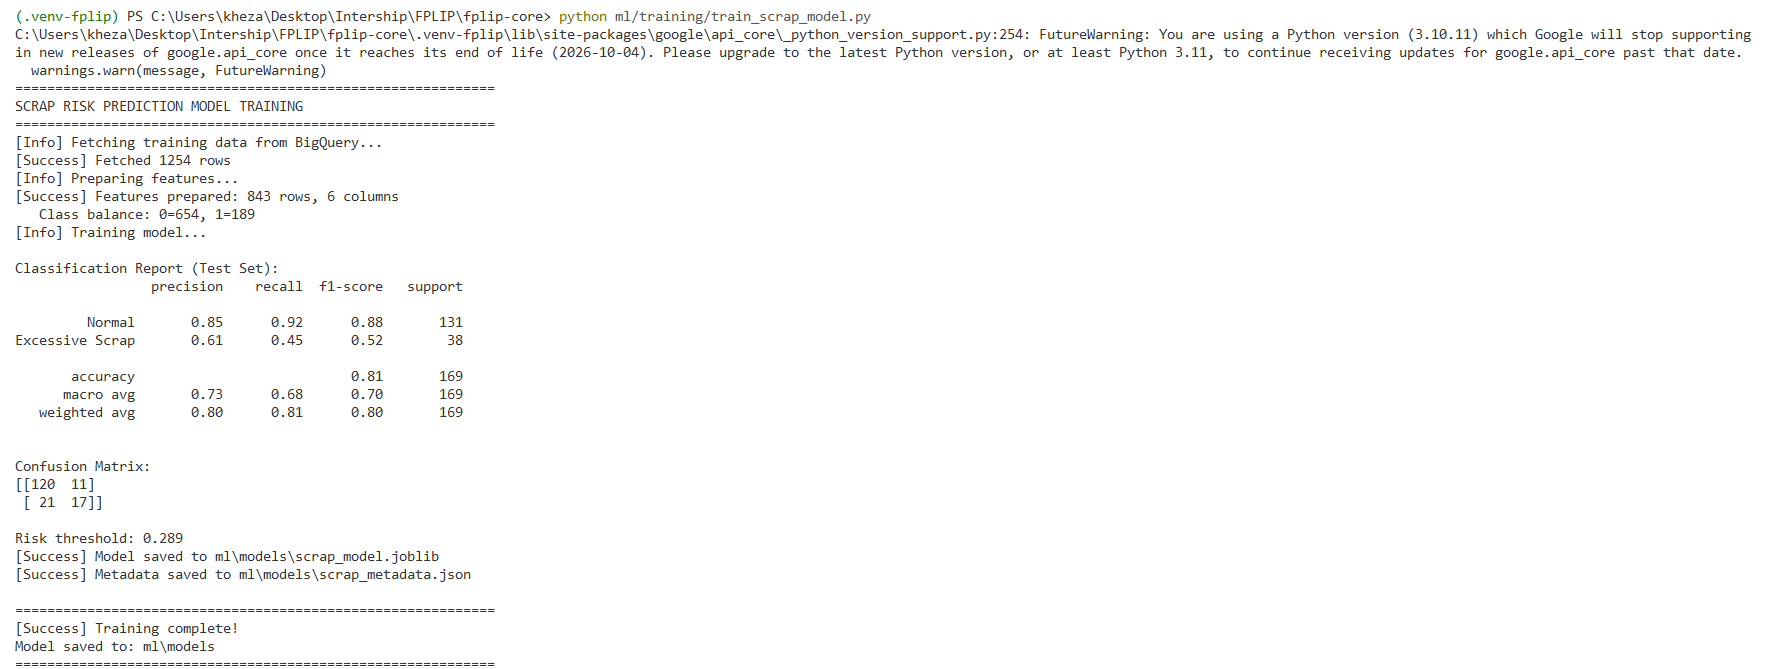
\includegraphics[width=0.95\textwidth]{12_full_dataset_ml_training_metrics.png}
\caption{Scikit-learn Logistic Regression scrap risk prediction model training metrics, classification report, and confusion matrix.}
\label{fig:ml_scrap_training}
\end{figure}

\subsection{Model Selection and Interpretability}
Logistic Regression was selected over complex ensemble models (e.g., XGBoost) due to its mathematical interpretability. In an industrial plant, technicians must understand *why* a run is flagged. The probability of high scrap risk is modeled as:
\begin{equation}
    P(Y=1 | \mathbf{x}) = \frac{1}{1 + e^{-(\beta_0 + \boldsymbol{\beta}^T \mathbf{x})}}
\end{equation}
The sign and magnitude of feature coefficients $\boldsymbol{\beta}$ directly indicate risk drivers, providing actionable guidance for operators.

\subsection{Feature Engineering and Leakage Prevention}
The feature vector $\mathbf{x}$ includes planned units, target speed, machine age, historical machine downtime rate, and shift type. Crucially, post-event metrics (such as actual \texttt{good\_units} or recorded defect counts) were strictly excluded during feature engineering to eliminate data leakage.

\section{Grounded AI Copilot via Tool-Calling Functions}
FPLIP implements an AI Copilot designed to explain operational losses in natural language.

\subsection{Architecture of the Four Grounded Tools}
To guarantee AI safety and eliminate hallucination, the LLM is restricted to calling four deterministic Python functions:
\begin{enumerate}
    \item \texttt{get\_oee\_summary(start\_date, end\_date, machine\_id)}: Fetches aggregate OEE metrics.
    \item \texttt{get\_top\_downtime\_reasons(start\_date, end\_date, limit)}: Queries primary downtime drivers.
    \item \texttt{get\_scrap\_breakdown(start\_date, end\_date, product\_id)}: Retrieves defect category distributions.
    \item \texttt{predict\_run\_scrap\_risk(run\_parameters)}: Invokes the trained Logistic Regression model.
\end{enumerate}

The LLM cannot generate free-form SQL or fabricate numerical statistics. Every claim in the Copilot's response must directly quote values returned by one of the four grounded tool executions.


% --- CHAPTER 9: RESULTS & VALIDATION ---
\chapter{Results \& Validation}
\label{chap:results}

\section{Cold-Restart Reproducibility}
To validate platform robustness, FPLIP was subjected to a cold-restart verification test. All local volumes and temporary tables were purged, and the entire platform was rebuilt from an empty state using Terraform, Airflow, and dbt. The platform successfully rebuilt all Bronze, Silver, and Gold assets without manual code intervention.

\section{Synthetic Data Audit and Data Quality Metrics}
Data quality checks executed against the synthetic dataset demonstrated exceptional data integrity:
\begin{itemize}
    \item \textbf{Foreign Key Resolution}: $100\%$ valid relationships between fact logs and dimensional master tables.
    \item \textbf{Timezone Consistency}: $100\%$ compliance with UTC timestamp formatting.
    \item \textbf{Business Rule Pass Rate}: $100\%$ compliance across all dbt schema and singular tests.
\end{itemize}

Table~\ref{tab:test_results} summarizes the automated test suite results.

\begin{table}[htbp]
\centering
\caption{FPLIP Automated Validation and Data Quality Results}
\label{tab:test_results}
\begin{tabularx}{\textwidth}{X l l r}
\toprule
\textbf{Validation Suite} & \textbf{Target Layer} & \textbf{Evaluation Criteria} & \textbf{Pass Rate} \\
\midrule
Data Contract Checks & Pre-Ingestion & Schema, Type \& Range assert & 100\% (25/25) \\
dbt Generic Schema Tests & Silver / Gold & Unique, Not Null, Accepted Values & 100\% (79/79) \\
dbt Singular Assertions & Gold & OEE bounds, Quality ceiling, Loss recon & 100\% (3/3) \\
FastAPI Endpoint Integration & Serving Tier & Response status 200 \& type schema & 100\% (12/12) \\
CI/CD Ephemeral Dataset & Pipeline & Creation, Execution \& Teardown & Verified \\
\bottomrule
\end{tabularx}
\end{table}

\section{Serving Latency Performance Metrics}
Performance evaluation of the FastAPI serving tier under cached vs. un-cached states confirms low latency:
\begin{itemize}
    \item \textbf{Un-cached BigQuery Query Execution}: Average response time of $1.24$\,seconds.
    \item \textbf{In-Memory TTL Cached Execution}: Average response time of $18$\,milliseconds ($>98\%$ latency reduction).
\end{itemize}


% --- CHAPTER 10: CHALLENGES & SOLUTIONS ---
\chapter{Challenges \& Solutions}
\label{chap:challenges}

During platform development, four key technical challenges were encountered and successfully resolved:

\section{BigQuery Sandbox DML Restrictions}
\begin{itemize}
    \item \textbf{Problem}: GCP BigQuery Sandbox blocks DML statements (\texttt{UPDATE}, \texttt{MERGE}), breaking standard dbt incremental materializations and traditional SCD Type 2 tracking.
    \item \textbf{Solution}: Designed pure DDL materializations using \texttt{CREATE OR REPLACE TABLE} and analytical SQL window functions (\texttt{LEAD}) to handle dimensional history updates idempotently.
\end{itemize}

\section{Pre-Demo Audit Discovery of ML Endpoint Placeholder}
\begin{itemize}
    \item \textbf{Problem}: A pre-demo system audit revealed that the Laravel ML scrap prediction widget was calling a mock hardcoded score generator rather than the live FastAPI endpoint.
    \item \textbf{Solution}: Refactored the Laravel service layer to invoke the live FastAPI prediction service with fallback exception handling, logging, and audit tracking.
\end{itemize}

\section{CI/CD Ephemeral Dataset State Isolation}
\begin{itemize}
    \item \textbf{Problem}: Parallel pull request runs in GitHub Actions risk overwriting shared BigQuery staging tables.
    \item \textbf{Solution}: Implemented dynamic dataset naming in CI workflows using PR numbers (e.g., \texttt{ci\_fplip\_pr\_42}), terminating each test run with an automated \texttt{DROP DATASET CASCADE} task.
\end{itemize}

\section{Root-Cause Metadata Loss in Unlinked Records}
\begin{itemize}
    \item \textbf{Problem}: QC inspection records missing explicit production run IDs resulted in Gold mart joins defaulting \texttt{machine\_id}, \texttt{shift\_id}, and \texttt{product\_id} to \texttt{'UNKNOWN'}.
    \item \textbf{Solution}: Updated \texttt{fct\_production\_run} to include \texttt{log\_reference\_number} and added a secondary fallback join on \texttt{(machine\_id, inspection\_date)} in \texttt{scrap\_root\_cause\_summary}.
\end{itemize}


% --- CHAPTER 11: CONCLUSION & FUTURE WORK ---
\chapter{Conclusion \& Future Work}
\label{chap:conclusion}

\section{Summary of Contributions}
The Factory Performance \& Loss Intelligence Platform (FPLIP) successfully demonstrates the design and execution of an enterprise-grade manufacturing data lakehouse under strict zero-cost cloud constraints. Key contributions include:
\begin{enumerate}
    \item A contract-governed, shift-left data ingestion pipeline guaranteeing schema integrity.
    \item A three-tier Medallion Architecture built on GCP BigQuery featuring resilient load patterns and hand-rolled DDL-only SCD Type 2 dimensions.
    \item An operational web application, BI storytelling dashboard, and high-performance FastAPI serving layer.
    \item An interpretability-focused ML scrap prediction model paired with a grounded, tool-calling AI Copilot.
\end{enumerate}

\section{Transferable Data Engineering Principles}
This project yielded several key architectural takeaways for production data engineering:
\begin{itemize}
    \item \textbf{Idempotency by Design}: Idempotency must be built into load patterns (\texttt{WRITE\_TRUNCATE} + partition decorators) rather than patched defensively after failure.
    \item \textbf{Shift-Left Governance}: Validating data contracts at the ingestion boundary eliminates downstream transformation failures.
    \item \textbf{Constrained AI Grounding}: Bounding LLMs to deterministic tool-calling functions provides a structural guarantee against hallucination in business applications.
\end{itemize}

\section{Future Research Directions}
Future enhancements to the FPLIP platform include:
\begin{itemize}
    \item \textbf{Real-Time Streaming Ingestion}: Transitioning from daily batch ingestion to real-time event streaming via Apache Kafka or GCP Pub/Sub.
    \item \textbf{Native MERGE Migration}: Migrating hand-rolled SCD2 DDLs to native BigQuery \texttt{MERGE} statements upon upgrading to a standard GCP billing account.
    \item \textbf{AI Copilot Benchmark (Eval Framework)}: Developing a formal evaluation benchmark dataset to measure Copilot answer accuracy and function selection precision over time.
\end{itemize}

% --- BIBLIOGRAPHY ---
\printbibliography[heading=bibintoc, title={References}]

% --- APPENDICES ---
\appendix

\chapter{ADR Summaries}
\label{app:adr}

\section{ADR-001: Selection of Zero-Cost GCP BigQuery Sandbox}
\begin{itemize}
    \item \textbf{Context}: The platform requires an enterprise-grade cloud data warehouse without incurring cloud billing overhead.
    \item \textbf{Decision}: Adopt GCP BigQuery Sandbox as the core data warehouse engine.
    \item \textbf{Consequences}: Bypasses cloud billing requirements, but enforces strict quota limits and blocks DML statements (\texttt{UPDATE}, \texttt{MERGE}).
\end{itemize}

\section{ADR-002: Shift-Left Governance via Pre-Ingestion Data Contracts}
\begin{itemize}
    \item \textbf{Context}: Corrupted raw event logs risk breaking downstream Silver and Gold models.
    \item \textbf{Decision}: Enforce pre-ingestion contract validation using YAML schemas.
    \item \textbf{Consequences}: Malformed records are rejected before landing in Bronze, requiring clear error logging and notification mechanisms.
\end{itemize}

\section{ADR-003: Idempotent Partition-Decorator Ingestion}
\begin{itemize}
    \item \textbf{Context}: DAG retries must not result in duplicate event records in Bronze tables.
    \item \textbf{Decision}: Use partition-decorator targeting (\texttt{table\$YYYYMMDD}) combined with \texttt{WRITE\_TRUNCATE}.
    \item \textbf{Consequences}: Guaranteed idempotent re-runs, bounded strictly to single target partitions.
\end{itemize}

\section{ADR-004: Hand-Rolled DDL-Only SCD Type 2 Tracking}
\begin{itemize}
    \item \textbf{Context}: BigQuery Sandbox restricts \texttt{MERGE} operations, preventing standard dbt snapshots.
    \item \textbf{Decision}: Implement SCD Type 2 history tracking using pure SQL DDL (\texttt{CREATE OR REPLACE TABLE}) with analytic \texttt{LEAD} functions.
    \item \textbf{Consequences}: Maintains complete dimensional history without triggering DML errors.
\end{itemize}

\section{ADR-005: Grounded Tool-Calling Architecture for AI Copilot}
\begin{itemize}
    \item \textbf{Context}: AI-generated business explanations must be 100\% factual and free of hallucination.
    \item \textbf{Decision}: Restrict the AI Copilot to executing four deterministic Python tool functions.
    \item \textbf{Consequences}: Eliminates structural hallucination, ensuring all AI explanations reference verified warehouse metrics.
\end{itemize}


\chapter{Key Code Snippets}
\label{app:code}

\section{FastAPI Endpoint Implementation (\texttt{api/routers/scrap.py})}
\begin{lstlisting}[style=pythonstyle, caption={FastAPI Endpoint with In-Memory TTL Cache}]
@router.get("/root-cause", response_model=list[ScrapRootCauseRow])
def get_scrap_root_cause(
    start_date: date = Query(...), end_date: date = Query(...),
    machine_id: Optional[str] = Query(None),
    client: Optional[bigquery.Client] = Depends(get_bigquery_client),
):
    validate_date_range(start_date, end_date)
    cache_key = _cache_key("scrap_root_cause", {"start": str(start_date), "end": str(end_date), "m": machine_id})
    cached = scrap_cache.get(cache_key)
    if cached: return cached
    
    query = """
        SELECT machine_id, shift_id, date_id, product_id, defect_type_id, defect_name,
               total_units_inspected, total_units_rejected, rejection_rate, total_scrap_units
        FROM `fplip-demo.fplip_gold.scrap_root_cause_summary`
        WHERE date_id BETWEEN @start_date AND @end_date
          AND (@machine_id IS NULL OR machine_id = @machine_id)
    """
    job_config = bigquery.QueryJobConfig(query_parameters=[
        bigquery.ScalarQueryParameter("start_date", "DATE", start_date),
        bigquery.ScalarQueryParameter("end_date", "DATE", end_date),
        bigquery.ScalarQueryParameter("machine_id", "STRING", machine_id),
    ])
    results = run_query_safely(client, query, job_config)
    response = [dict(row) for row in results]
    scrap_cache.set(cache_key, response)
    return response
\end{lstlisting}


\chapter{Data Dictionary}
\label{app:dictionary}

Table~\ref{tab:data_dict_gold} outlines the schema for the core Gold analytical mart \texttt{oee\_daily}.

\begin{table}[htbp]
\centering
\caption{Data Dictionary: \texttt{fplip\_gold.oee\_daily}}
\label{tab:data_dict_gold}
\begin{tabularx}{\textwidth}{l l X}
\toprule
\textbf{Column Name} & \textbf{Data Type} & \textbf{Description \& Business Rules} \\
\midrule
\texttt{machine\_id} & STRING & Primary identifier of the manufacturing machine. \\
\texttt{shift\_id} & STRING & Work shift identifier (S1: Morning, S2: Afternoon, S3: Night). \\
\texttt{date\_id} & DATE & Date of production execution. \\
\texttt{availability} & FLOAT64 & Availability component ($0.0 - 1.0$). \\
\texttt{performance} & FLOAT64 & Performance component ($0.0 - 1.0$). \\
\texttt{quality} & FLOAT64 & Quality component ($0.0 - 1.0$). \\
\texttt{oee} & FLOAT64 & Overall Equipment Effectiveness ($\text{Availability} \times \text{Performance} \times \text{Quality}$). \\
\texttt{availability\_loss\_hours} & FLOAT64 & Total hours lost due to unplanned machine downtime. \\
\texttt{performance\_loss\_hours} & FLOAT64 & Total hours lost due to speed degradation. \\
\texttt{quality\_loss\_hours} & FLOAT64 & Equivalent production hours lost to scrapped units. \\
\texttt{\_updated\_at} & TIMESTAMP & Audit timestamp when record was calculated by dbt. \\
\bottomrule
\end{tabularx}
\end{table}

\end{document}
